%!Mode:: "TeX:UTF-8"
\documentclass[a4paper,11pt,UTF8]{ctexart}

\usepackage{indentfirst} %缩进
\usepackage{xeCJK}    %使用系统字体
\usepackage{fancyhdr} %自定义页眉页脚
\pagestyle{empty}                   %不设置页眉页脚
\usepackage{amsmath, amsthm, amssymb, amsfonts} %数学公式
\usepackage[a4paper,left=3cm,right=3cm,top=3cm,bottom=3cm]{geometry}
%\usepackage[tmargin=1in,bmargin=1in,lmargin=1.25in,rmargin=1.25in]{geometry}.
\usepackage{booktabs} %插入表格
\usepackage[section]{placeins} %避免浮动
\usepackage{listings} %插入代码
\usepackage{ctex}     %中文宏包
\usepackage[svgnames, table]{xcolor} %彩色表格
\usepackage{algorithm}          %伪代码
\usepackage{algorithmicx}
\usepackage{algpseudocode}
\usepackage{algorithm,algpseudocode,float}
\usepackage{lipsum}
\usepackage{enumitem}           %调整列举环境
\usepackage{url}
\usepackage{fontspec,xunicode}
\defaultfontfeatures{Mapping=tex-text} %如果没有它,会有一些 tex 特殊字符无法正常使用,比如连字符。

\usepackage{graphicx}
\graphicspath{{imgs/}}

\usepackage{upgreek}

%%%%%%%%%%%%%%%%%%%%%%%%%%%%%%%%%%%%%%%%%%%%%%%%%%%%%%%%%%%%%%%%
% 缩进及行间距
%%%%%%%%%%%%%%%%%%%%%%%%%%%%%%%%%%%%%%%%%%%%%%%%%%%%%%%%%%%%%%%%
\setlength{\parindent}{22pt} %重新定义缩进长度
\setlength{\baselineskip}{20pt}  %定义行间距
%\renewcommand{\baselinestretch}{1.1} %定义行间距

%%%%%%%%%%%%%%%%%%%%%%%%%%%%%%%%%%%%%%%%%%%%%%%%%%%%%%%%%%%%%%%%
% 列表设置
%%%%%%%%%%%%%%%%%%%%%%%%%%%%%%%%%%%%%%%%%%%%%%%%%%%%%%%%%%%%%%%%
\setenumerate{fullwidth,itemindent=\parindent,listparindent=\parindent,itemsep=0ex,partopsep=0pt,parsep=0ex}
\setenumerate[2]{label=\alph*),leftmargin=1.5em}  %二级item设置
\setitemize{itemindent=38pt,leftmargin=0pt,itemsep=-0.4ex,listparindent=26pt,partopsep=0pt,parsep=0.5ex,topsep=-0.25ex}
\setdescription{itemindent=38pt,leftmargin=0pt,itemsep=-0.4ex,listparindent=26pt,partopsep=0pt,parsep=0.5ex,topsep=-0.25ex}

%%%%%%%%%%%%%%%%%%%%%%%%%%%%%%%%%%%%%%%%%%%%%%%%%%%%%%%%%%%%%%%%
% 图的标题行间距设置
%%%%%%%%%%%%%%%%%%%%%%%%%%%%%%%%%%%%%%%%%%%%%%%%%%%%%%%%%%%%%%%%
\newcommand{\bottomcaption}{%
\setlength{\abovecaptionskip}{6pt}%
\setlength{\belowcaptionskip}{6pt}%
\caption}


%%%%%%%%%%%%%%%%%%%%%%%%%%%%%%%%%%%%%%%%%%%%%%%%%%%%%%%%%%%%%%%%
% 字体定义
%%%%%%%%%%%%%%%%%%%%%%%%%%%%%%%%%%%%%%%%%%%%%%%%%%%%%%%%%%%%%%%%
\setmainfont{Times New Roman}  %默认英文字体.serif是有衬线字体sans serif无衬线字体
\setmonofont{Consolas}
\setCJKmainfont[ItalicFont={楷体}, BoldFont={黑体}]{宋体}%衬线字体 缺省中文字体为
\setCJKsansfont{黑体}
\punctstyle{hangmobanjiao}
%-----------------------xeCJK下设置中文字体------------------------------%
\setCJKfamilyfont{song}{SimSun}                             %宋体 song
\newcommand{\song}{\CJKfamily{song}}
\setCJKfamilyfont{fs}{FangSong}                      %仿宋  fs
\newcommand{\fs}{\CJKfamily{fs}}
\setCJKfamilyfont{ktgb}{KaiTi}                      %楷体2312 ktgb
\newcommand{\ktgb}{\CJKfamily{ktgb}}
\setCJKfamilyfont{yh}{Microsoft YaHei}                    %微软雅黑 yh
\newcommand{\yh}{\CJKfamily{yh}}
\setCJKfamilyfont{hei}{SimHei}                              %黑体  hei
\newcommand{\hei}{\CJKfamily{hei}}
\setCJKfamilyfont{hwxk}{STXingkai}                                %华文行楷  hwxk
\newcommand{\hwxk}{\CJKfamily{hwxk}}
%------------------------------设置字体大小------------------------%
\newcommand{\shiyanbaogao}{\fontsize{36pt}{\baselineskip}\selectfont}
\newcommand{\chuhao}{\fontsize{42pt}{\baselineskip}\selectfont}     %初号
\newcommand{\xiaochuhao}{\fontsize{36pt}{\baselineskip}\selectfont} %小初号
\newcommand{\yihao}{\fontsize{28pt}{\baselineskip}\selectfont}      %一号
\newcommand{\erhao}{\fontsize{21pt}{\baselineskip}\selectfont}      %二号
\newcommand{\xiaoerhao}{\fontsize{18pt}{\baselineskip}\selectfont}  %小二号
\newcommand{\sanhao}{\fontsize{15.75pt}{\baselineskip}\selectfont}  %三号
\newcommand{\sihao}{\fontsize{14pt}{\baselineskip}\selectfont}       %四号
\newcommand{\xiaosihao}{\fontsize{12pt}{\baselineskip}\selectfont}  %小四号
\newcommand{\wuhao}{\fontsize{10.5pt}{\baselineskip}\selectfont}    %五号
\newcommand{\xiaowuhao}{\fontsize{9pt}{\baselineskip}\selectfont}   %小五号
\newcommand{\liuhao}{\fontsize{7.875pt}{\baselineskip}\selectfont}  %六号
\newcommand{\qihao}{\fontsize{5.25pt}{\baselineskip}\selectfont}    %七号

%%%%%%%%%%%%%%%%%%%%%%%%%%%%%%%%%%%%%%%%%%%%%%%%%%%%%%%%%%%%%%%%
% 图题字体大小相同
%%%%%%%%%%%%%%%%%%%%%%%%%%%%%%%%%%%%%%%%%%%%%%%%%%%%%%%%%%%%%%%%
\usepackage{caption}
\captionsetup{font={footnotesize}}   % footnotesize = 9pt
\captionsetup[lstlisting]{font={footnotesize}}

%%%%%%%%%%%%%%%%%%%%%%%%%%%%%%%%%%%%%%%%%%%%%%%%%%%%%%%%%%%%%%%%
% 重定义枚举编号为 1),2)...
%%%%%%%%%%%%%%%%%%%%%%%%%%%%%%%%%%%%%%%%%%%%%%%%%%%%%%%%%%%%%%%%
\renewcommand{\labelenumi}{\theenumi)}

%%%%%%%%%%%%%%%%%%%%%%%%%%%%%%%%%%%%%%%%%%%%%%%%%%%%%%%%%%%%%%%%
% 标题名称中文化
%%%%%%%%%%%%%%%%%%%%%%%%%%%%%%%%%%%%%%%%%%%%%%%%%%%%%%%%%%%%%%%%
\renewcommand\figurename{\hei 图}
\renewcommand\tablename{\hei 表}
\renewcommand\lstlistingname{\hei 代码}
\renewcommand{\algorithmicrequire}{\textbf{输入:}}
\renewcommand{\algorithmicensure}{\textbf{输出:}}
\newtheorem{define}{定义}

%%%%%%%%%%%%%%%%%%%%%%%%%%%%%%%%%%%%%%%%%%%%%%%%%%%%%%%%%%%%%%%%
% 代码设置
%%%%%%%%%%%%%%%%%%%%%%%%%%%%%%%%%%%%%%%%%%%%%%%%%%%%%%%%%%%%%%%%
\lstset{
 columns=fixed,
 numbers=left,                                        % 在左侧显示行号
 numberstyle=\tiny\color{gray},                       % 设定行号格式
 frame=single,                                        % 单线背景边框
 breaklines=true,                                     % 设定LaTeX对过长的代码行进行自动换行
 keywordstyle=\color[RGB]{40,40,255},                 % 设定关键字颜色
 numberstyle=\footnotesize\color{darkgray},
 commentstyle=\it\color[RGB]{0,96,96},                % 设置代码注释的格式
 stringstyle=\rmfamily\slshape\color[RGB]{128,0,0},   % 设置字符串格式
 showstringspaces=false,                              % 不显示字符串中的空格
 language=java,                                        % 设置语言
 basicstyle=\linespread{1.0}\xiaowuhao\ttfamily,                      % 字体字号
 %lineskip=10pt,
 %baselinestretch=1,
}

%%%%%%%%%%%%%%%%%%%%%%%%%%%%%%%%%%%%%%%%%%%%%%%%%%%%%%%%%%%%%%%%
% 伪代码分页
%%%%%%%%%%%%%%%%%%%%%%%%%%%%%%%%%%%%%%%%%%%%%%%%%%%%%%%%%%%%%%%%
\makeatletter
\renewcommand{\ALG@name}{算法}
\newenvironment{breakablealgorithm}
  {% \begin{breakablealgorithm}
   \begin{center}
     \refstepcounter{algorithm}% New algorithm
     \hrule height.8pt depth0pt \kern2pt% \@fs@pre for \@fs@ruled
     \renewcommand{\caption}[2][\relax]{% Make a new \caption
       {\raggedright\textbf{\ALG@name~\thealgorithm} ##2\par}%
       \ifx\relax##1\relax % #1 is \relax
         \addcontentsline{loa}{algorithm}{\protect\numberline{\thealgorithm}##2}%
       \else % #1 is not \relax
         \addcontentsline{loa}{algorithm}{\protect\numberline{\thealgorithm}##1}%
       \fi
       \kern2pt\hrule\kern2pt
     }
  }{% \end{breakablealgorithm}
     \kern2pt\hrule\relax% \@fs@post for \@fs@ruled
   \end{center}
  }
\makeatother

% =============================================
% Part 1 Edit the info
% =============================================

\newcommand{\major}{物理学院}
\newcommand{\name}{黄阅迅,李秋阳}
\newcommand{\stuid}{PB18020631,PB18020567}
\newcommand{\group}{20}
\newcommand{\newdate}{\today}


\newcommand{\course}{电子线路实验(1)}
\newcommand{\newtitle}{电压比较器及其应用实验}

%==============================================
%otheres
%==============================================
\newcommand\mr[1]{\mathrm{#1}}

% =============================================
% Part 1 Main document
% =============================================
\begin{document}
\thispagestyle{empty}
\begin{figure}[h]
  \begin{minipage}{0.6\linewidth}
    \centerline{
\includegraphics[width=\linewidth]{logo.png}}
  \end{minipage}
  \hfill
  \begin{minipage}{.4\linewidth}
    \raggedleft
    \begin{tabular*}{.8\linewidth}{ll}
      学院: & \underline\major   \\
      姓名: & \underline\name    \\
      学号: & \underline\stuid   \\
      组号:  & \underline\group   \\
      日期: & \underline\newdate \\
    \end{tabular*}
  \end{minipage}
\end{figure}

\begin{table}[!htbp]
  \centering
  \begin{tabular*}{\linewidth}{llllll}
    课程名称:  \underline\course   \qquad\qquad 实验题目:  \underline\newtitle  
  \end{tabular*}
\end{table}

% =============================================
% Part 2 Main document
% =============================================

\section{实验目的}

请参看预习报告。

\section{实验原理}

请参看预习报告。

\section{实验内容与步骤}
\subsection{实验一:单限比较器}
	实验电路图如图\ref{fig:Exp01}所示:
	\begin{figure}[H]
	 \centering
	 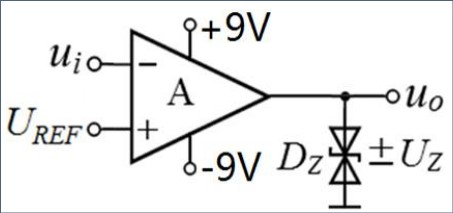
\includegraphics[width=5cm]{Exp01}
	 \caption{实验一电路图}
	 \label{fig:Exp01}
	\end{figure}
	$D_Z$ 为双向稳压管 2DW231 ,其稳定电压为 $U_Z=\pm 6\mr{V}$ 。输入信号为 $u_i=12\mr{V_{pp}}$ 、 $200\mr{Hz}$ 的三角波,用不同的比较电压 $U_{REF}$ 进行实验:
	\begin{enumerate}
	 \item $U_{REF}=0$ 。记录示波器输入输出波形,并用示波器 X-Y 模式绘制李萨如图形,记录输入输出特性曲线。
	 \item 仅 $U_{REF}=+5\mr{V}$ ,后续操作一致。
	 \item 仅 $U_{REF}=-5\mr{V}$ ,后续操作一致。
	\end{enumerate}
\subsection{实验二:窗口比较器}
	实验电路图如图\ref{fig:Exp02}所示:
	\begin{figure}[H]
	 \centering
	 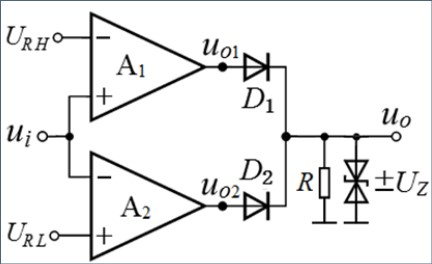
\includegraphics[width=5cm]{Exp02}
	 \caption{实验二电路图}
	 \label{fig:Exp02}
	\end{figure}
	$R=10\mr{k}\Omega$ , $U_Z=\pm 6\mr{V}$ ,$D_1,~D_2$ 为开关二极管。输入信号为 $u_i=12\mr{V_{pp}}$ 、 $200\mr{Hz}$ 的三角波。  $U_{RH}=+5\mr{V},~U_{RL}=-5\mr{V}$ 为高、低门限电压。记录示波器输入输出波形,并用示波器 X-Y 模式绘制李萨如图形,记录输入输出特性曲线。
\subsection{实验三:滞回比较器}
	实验电路图如图\ref{fig:Exp03}所示:
	\begin{figure}[H]
	 \centering
	 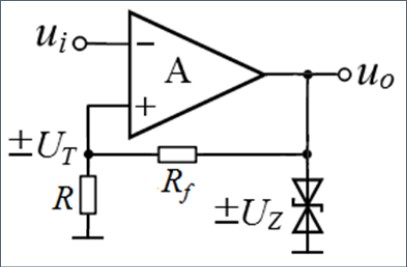
\includegraphics[width=5cm]{Exp03}
	 \caption{实验三电路图}
	 \label{fig:Exp03}
	\end{figure}
	$R=R_f=10\mr{k}\Omega$ , $U_Z=\pm 6\mr{V}$ 。输入信号为 $u_i=12\mr{V_{pp}}$ 、 $200\mr{Hz}$ 的三角波。记录示波器输入输出波形,并用示波器 X-Y 模式绘制李萨如图形,记录输入输出特性曲线。
\subsection{实验四:方波发生器(振荡器)}
	实验电路图如图\ref{fig:Exp04}所示:
	\begin{figure}[H]
	 \centering
	 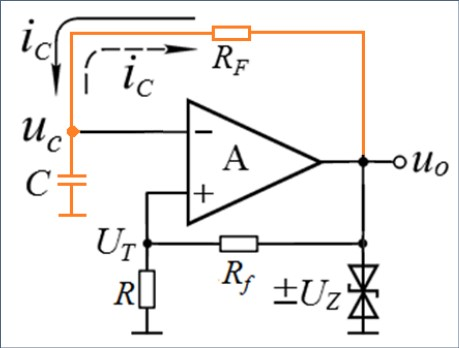
\includegraphics[width=5cm]{Exp04}
	 \caption{实验四电路图}
	 \label{fig:Exp04}
	\end{figure}
	$R=R_f=10\mr{k}\Omega$ , $R_F=24\mr{k}\Omega$ , $C=0.01\mr{\upmu F}$ , $U_Z=\pm 6\mr{V}$ 。仅接上芯片工作电压 $\pm9\mr{V}$ ,没有输入电压。记录示波器输入输出波形,并用示波器 X-Y 模式绘制李萨如图形,记录输入输出特性曲线。
	
\section{实验数据处理与分析}
\subsection{实验一:单限比较器}
	\subsubsection{实验数据}
		\begin{itemize}
		 \item 当 $U_{REF}=0$ 时:
		 \begin{figure}[H]
	 \centering
	 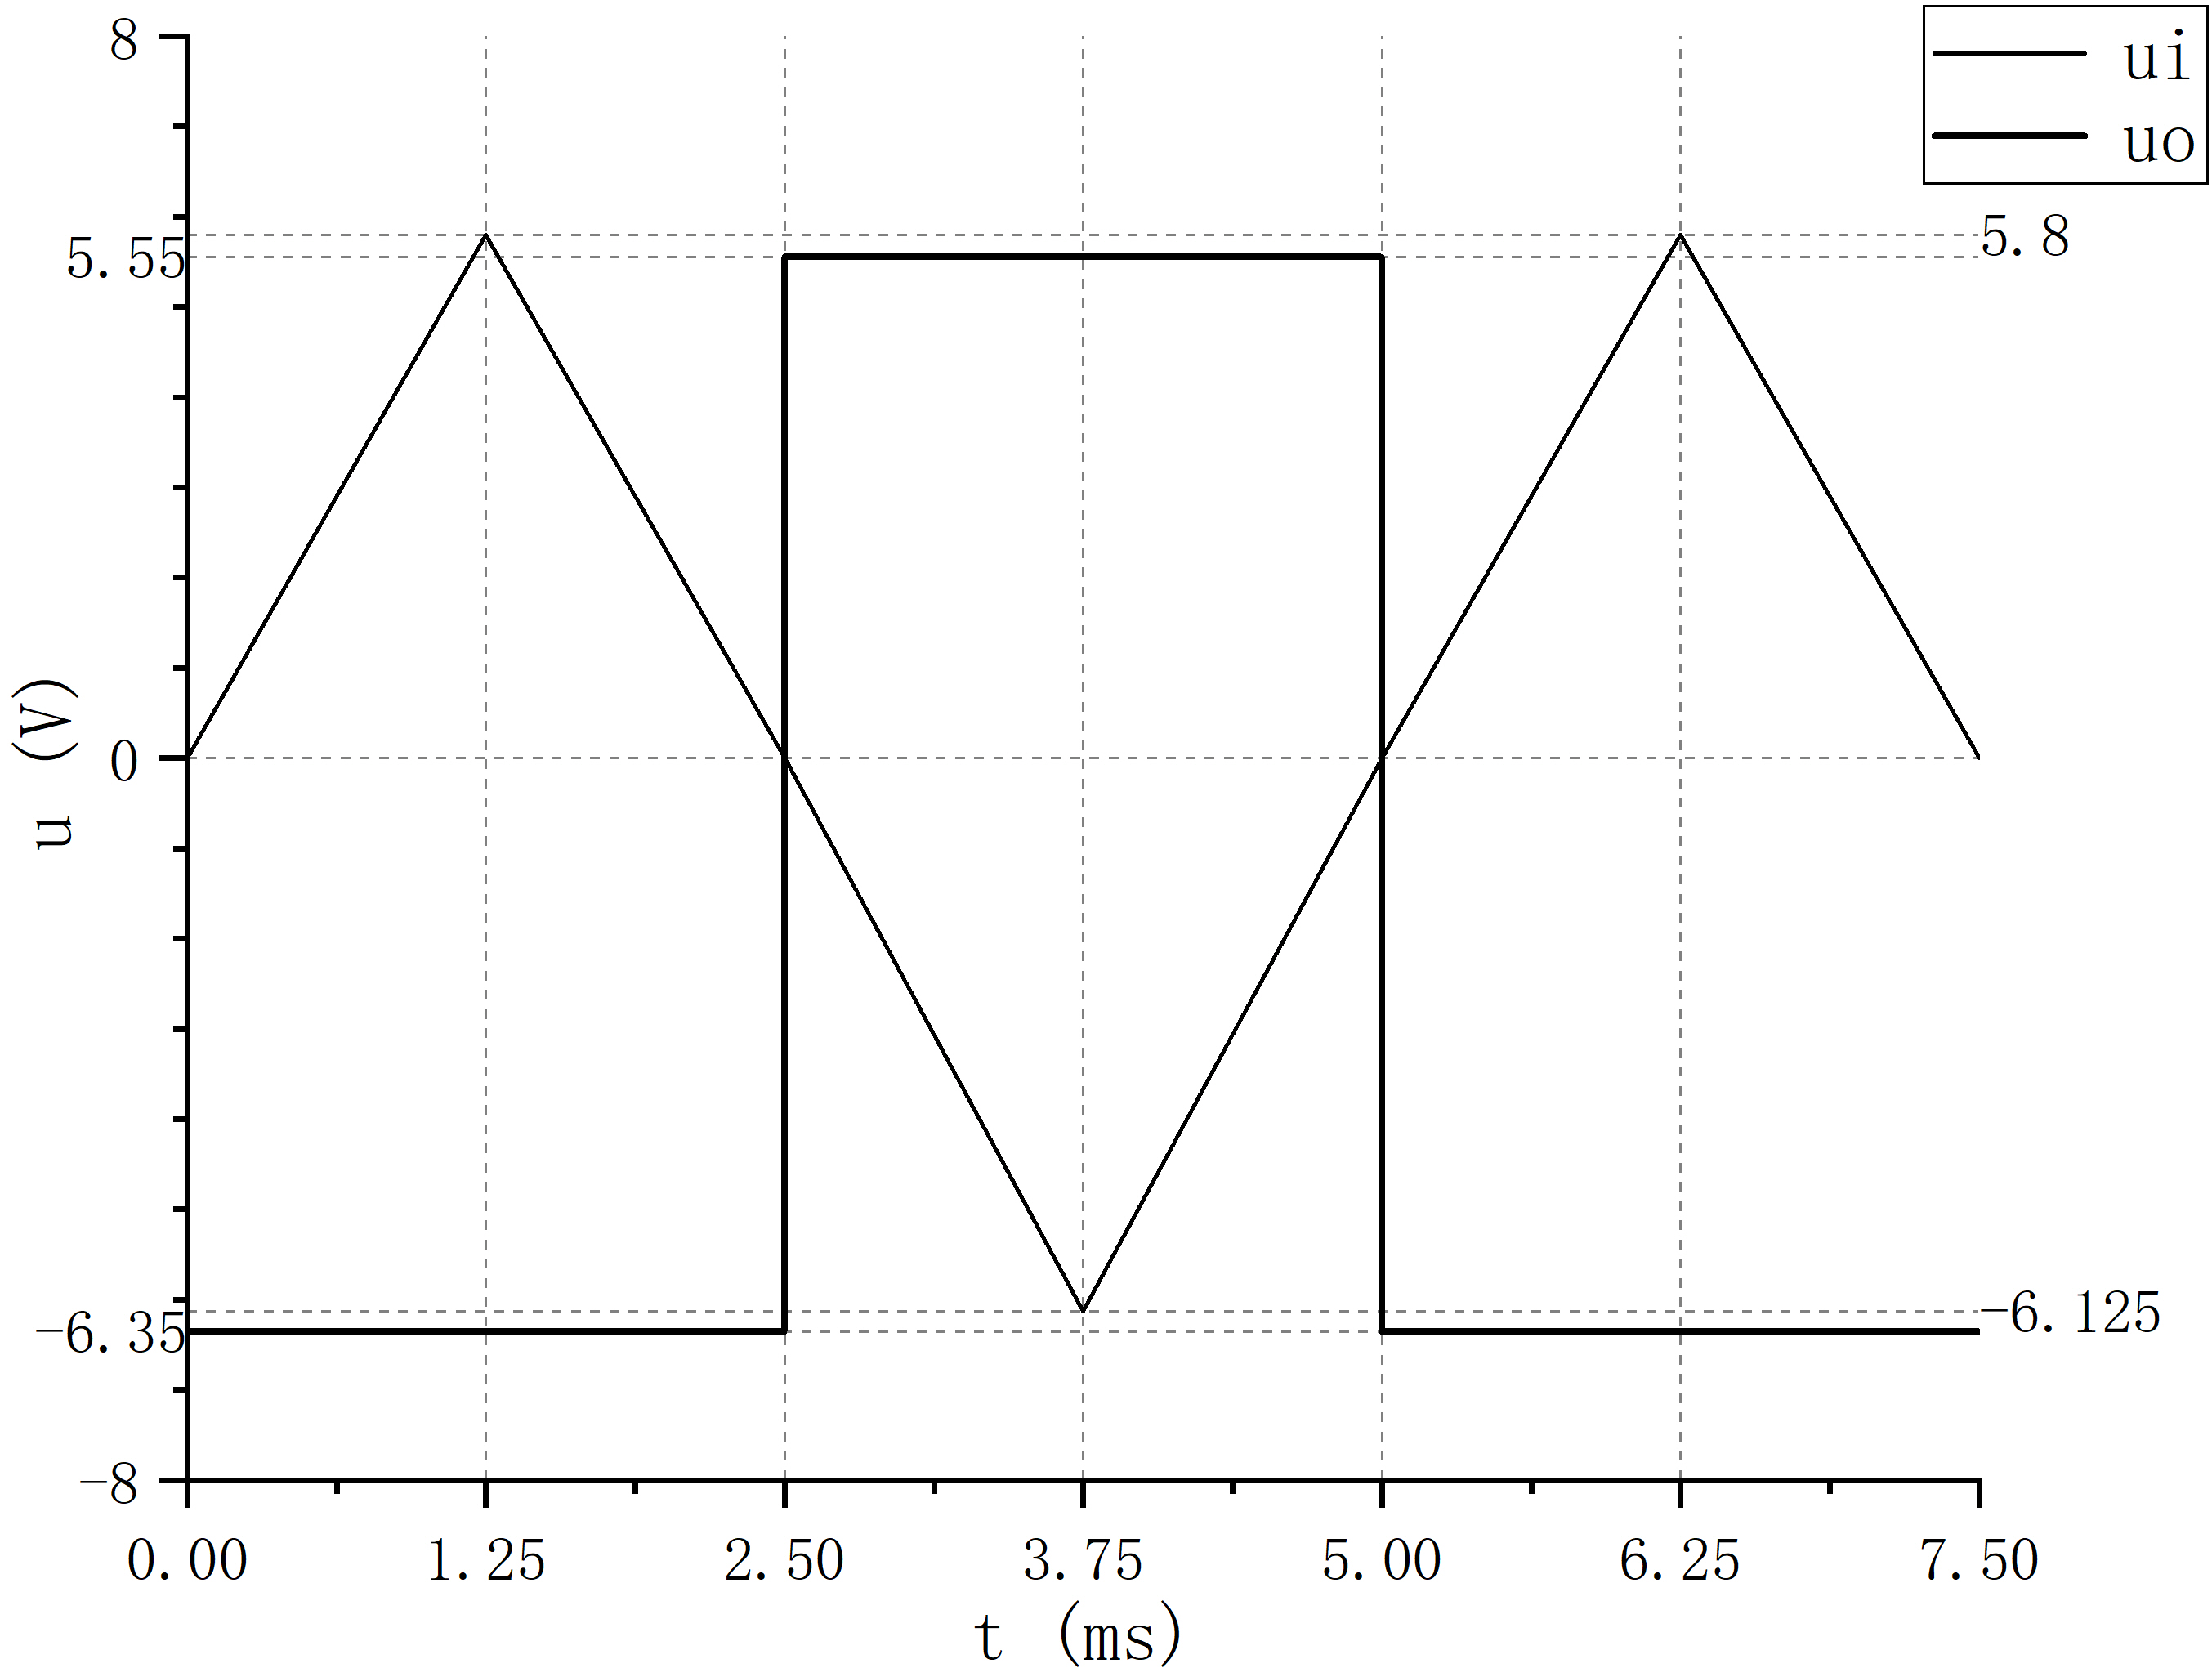
\includegraphics[width=8cm]{1-1-1}
	 \caption{实验一输入输出波形, $U_{REF}=0$}
	 \label{fig:1-1-1}
	\end{figure}
	\begin{figure}[H]
	 \centering
	 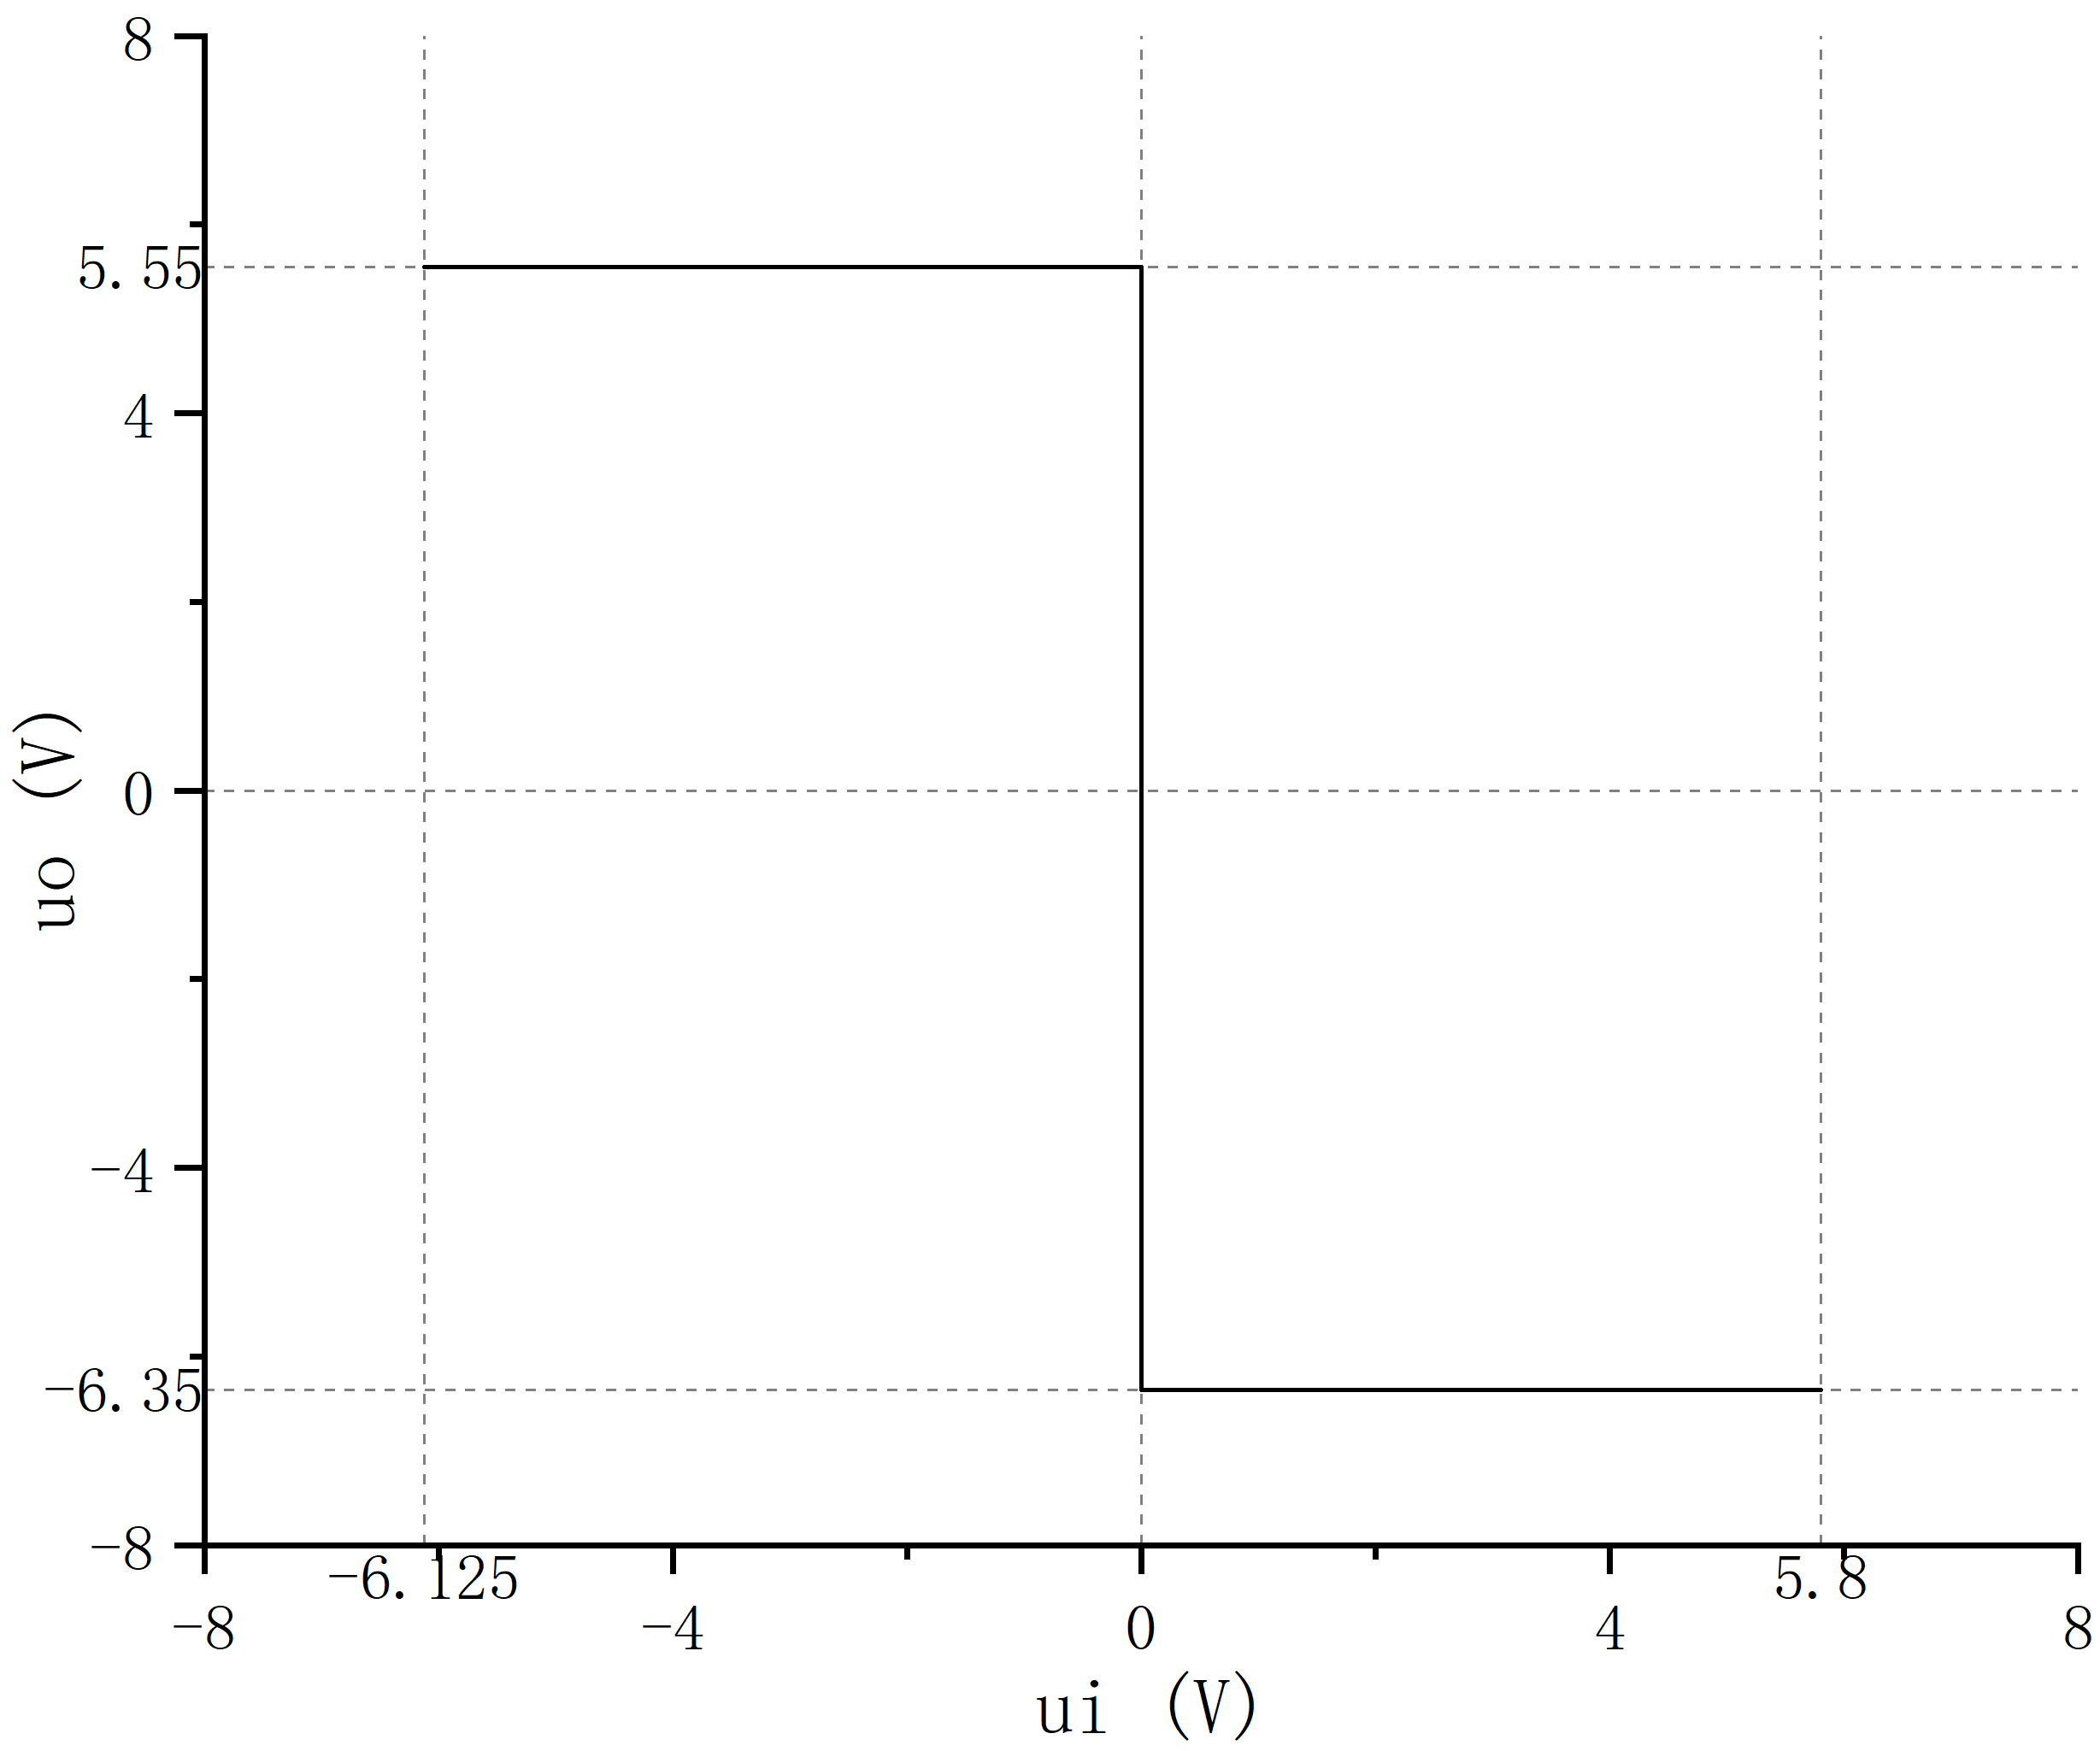
\includegraphics[width=8cm]{1-1-2}
	 \caption{实验一传输特性曲线, $U_{REF}=0$}
	 \label{fig:1-1-2}
	\end{figure}
	\item 当 $U_{REF}=+5\mr{V}$ 时:
		 \begin{figure}[H]
	 \centering
	 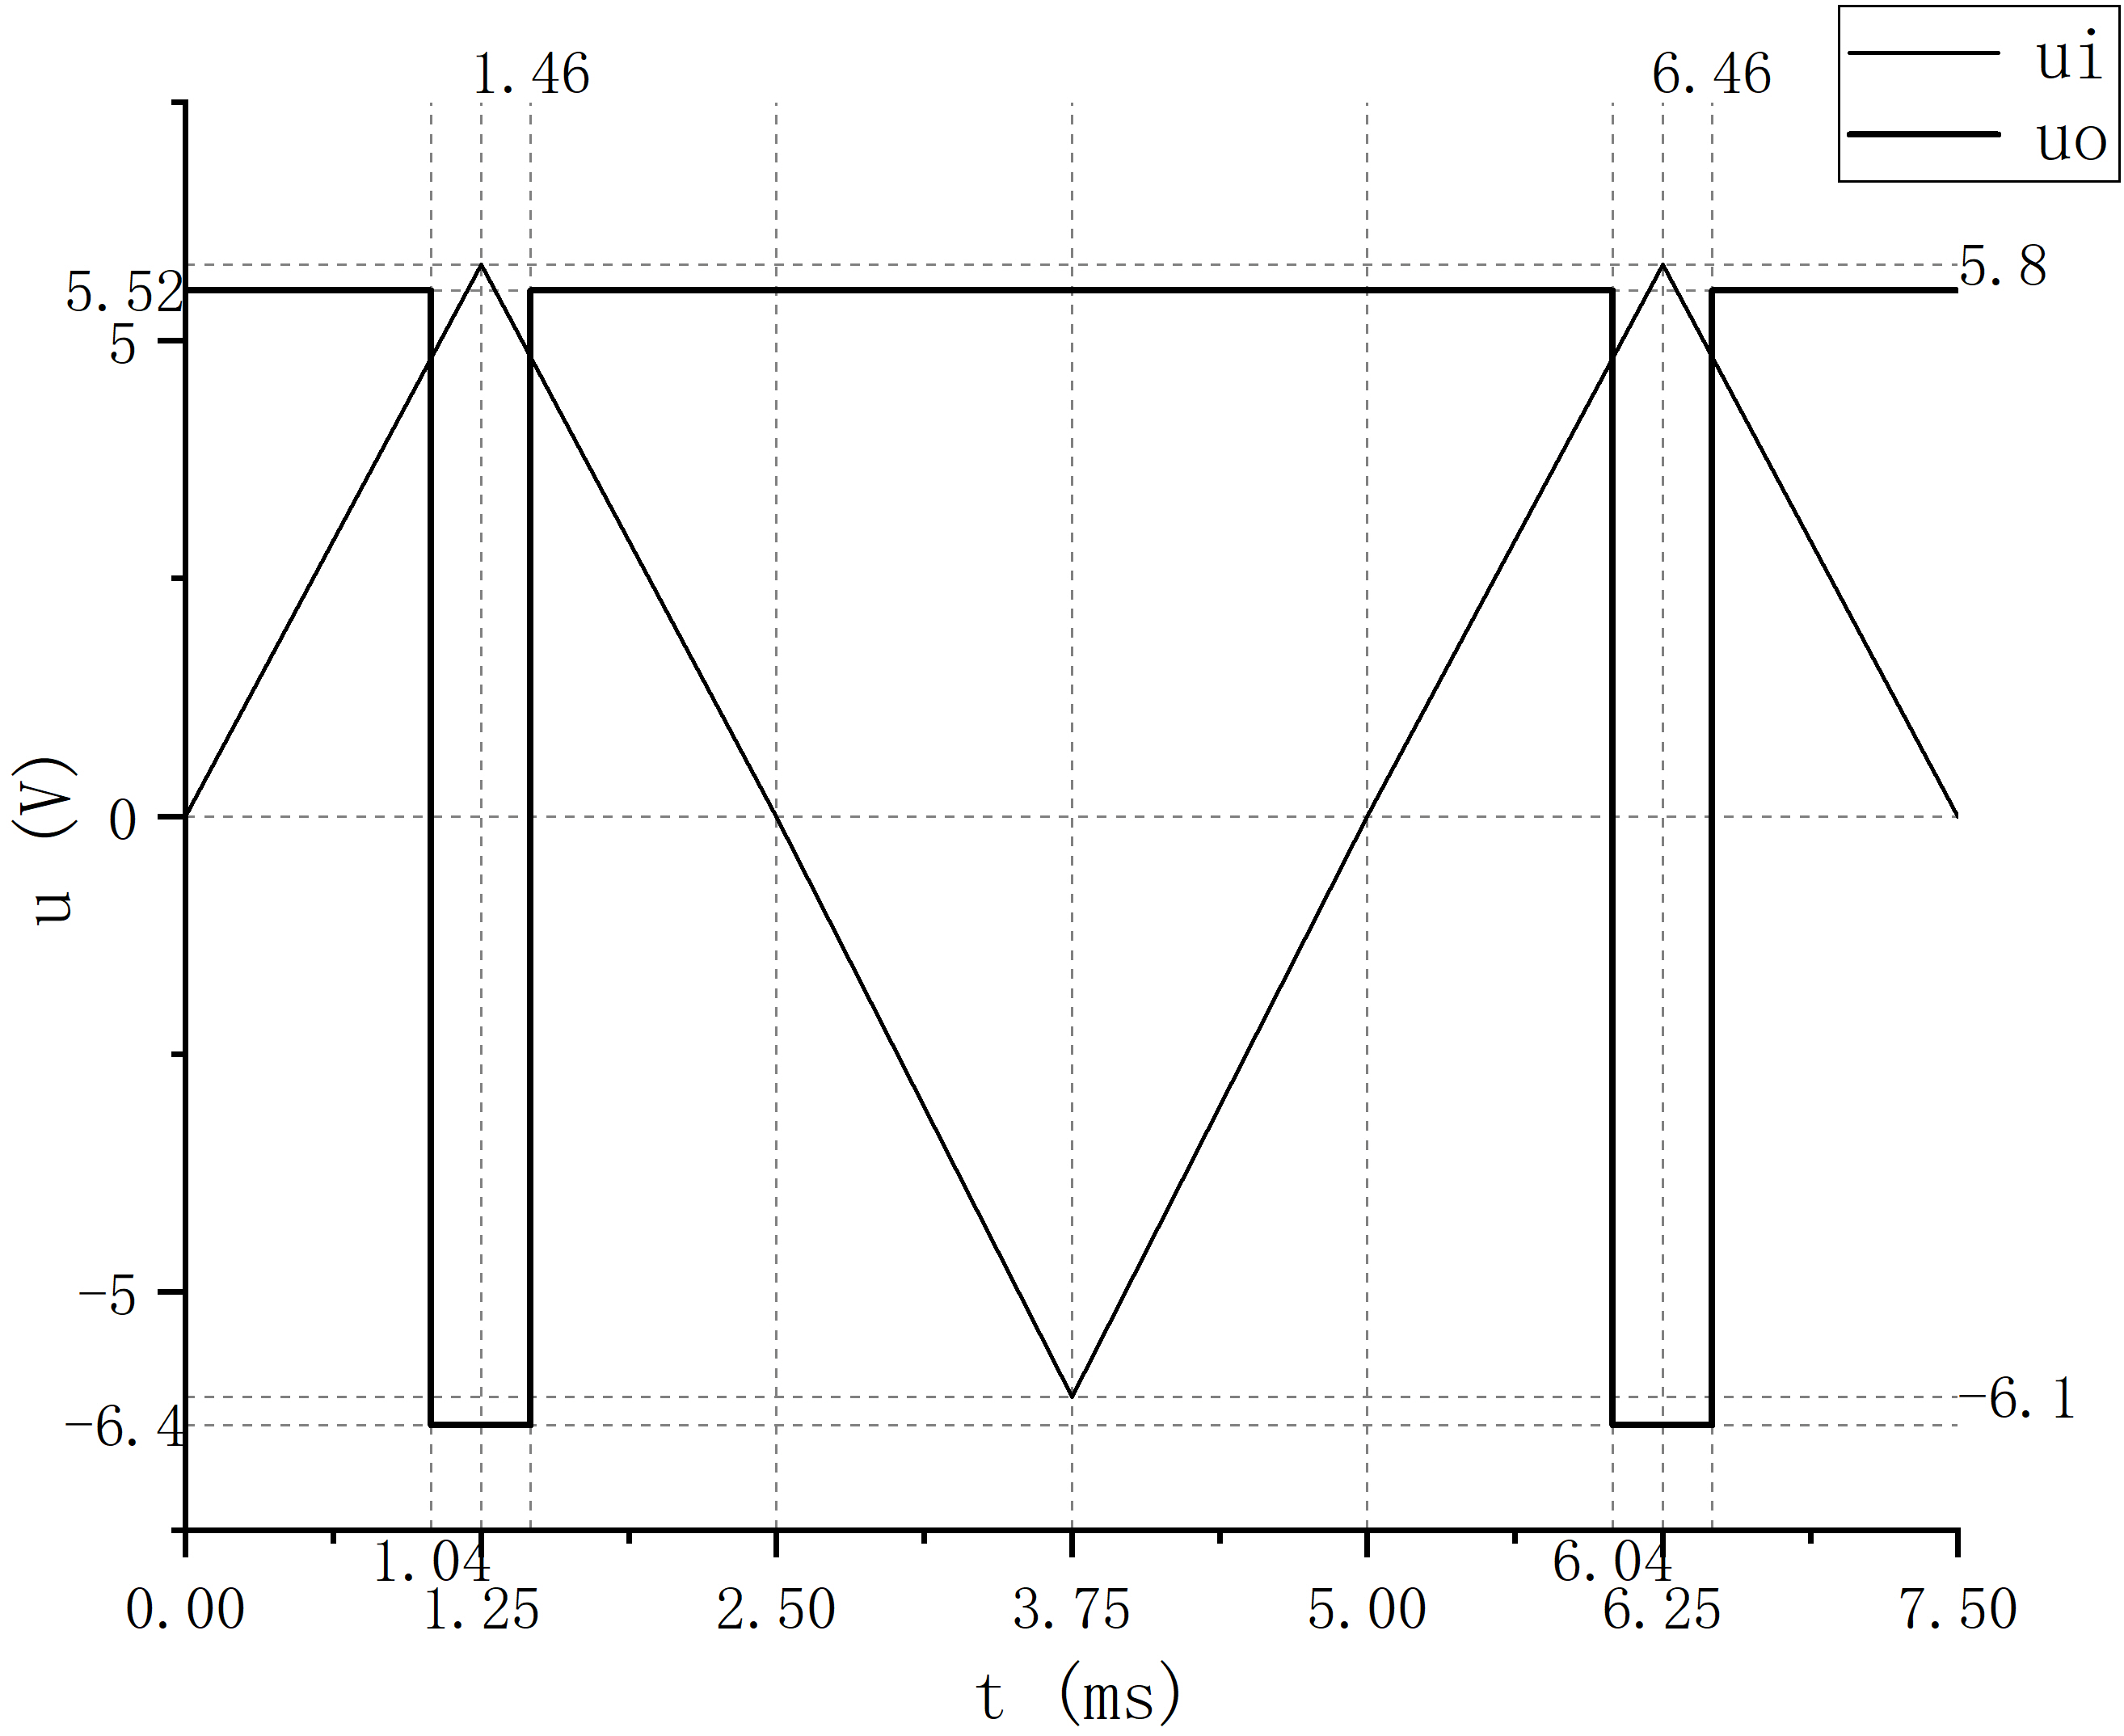
\includegraphics[width=8cm]{1-2-1}
	 \caption{实验一输入输出波形, $U_{REF}=+5\mr{V}$}
	 \label{fig:1-2-1}
	 \end{figure}
	 \begin{figure}[H]
	 	\centering
	 	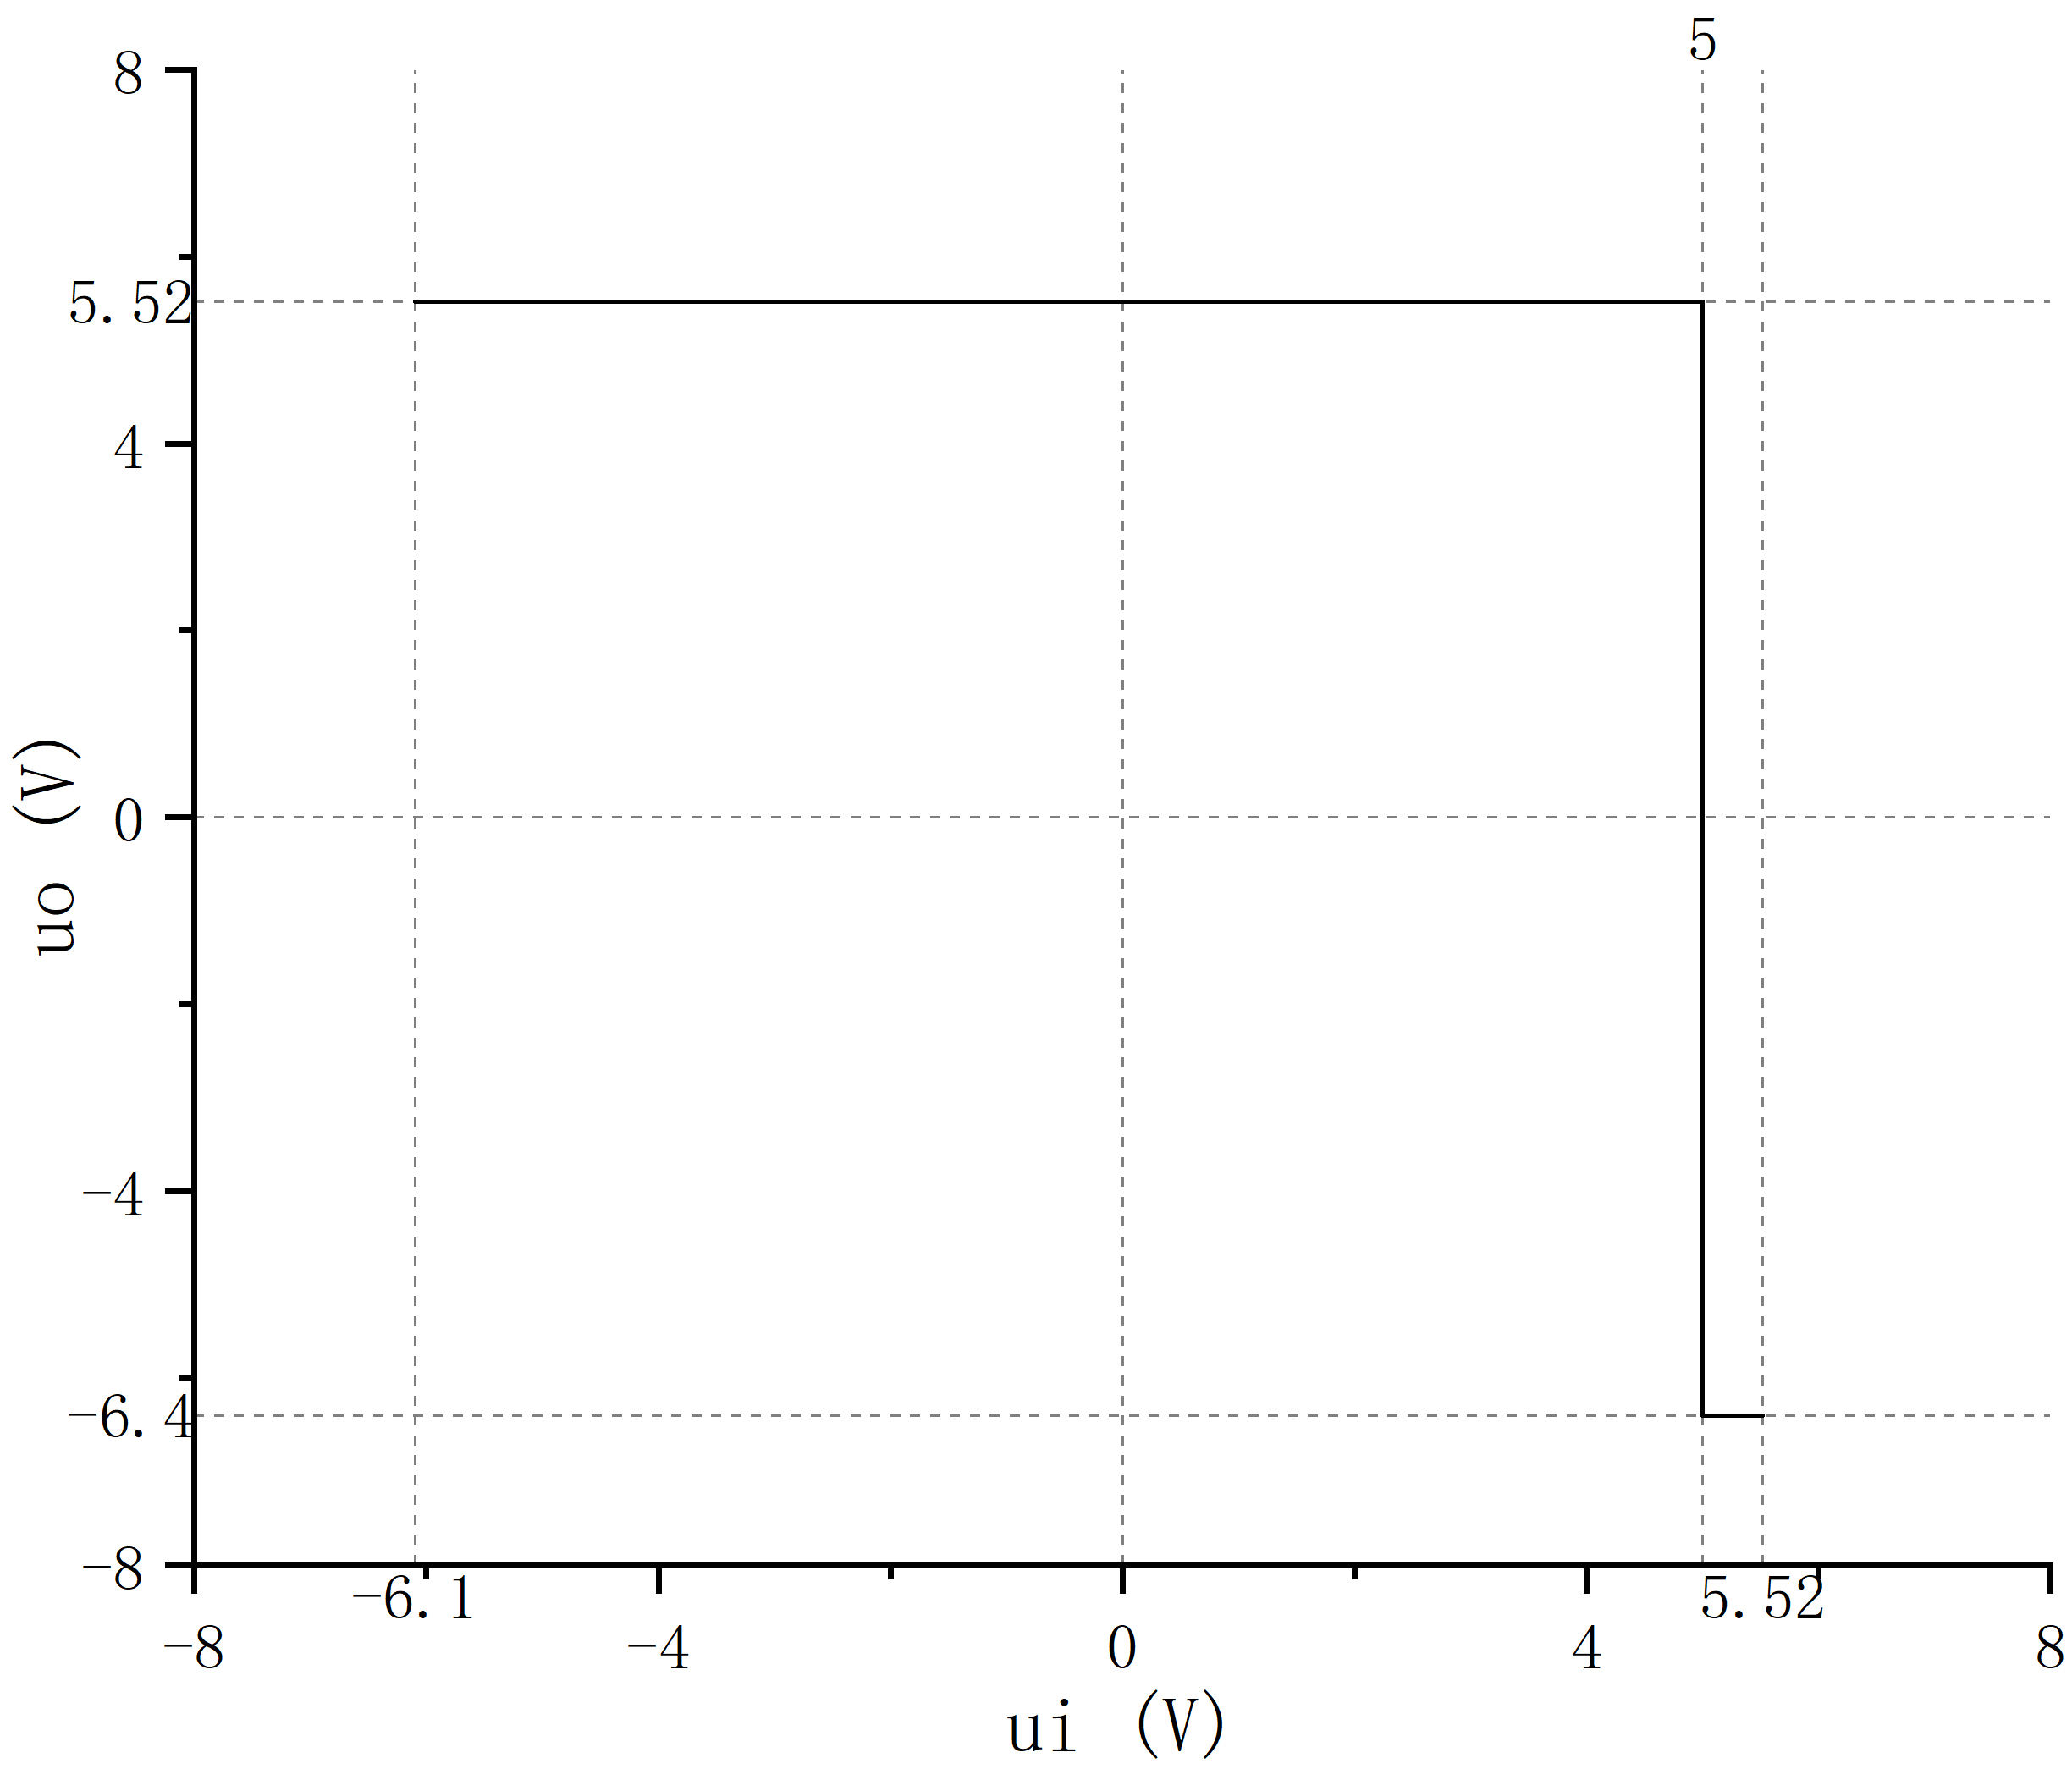
\includegraphics[width=8cm]{1-2-2}
		 \caption{实验一传输特性曲线, $U_{REF}=+5\mr{V}$}
		 \label{fig:1-2-2}
	 \end{figure}
	 \item 当 $U_{REF}=-5\mr{V}$ 时:
		 \begin{figure}[H]
	 \centering
	 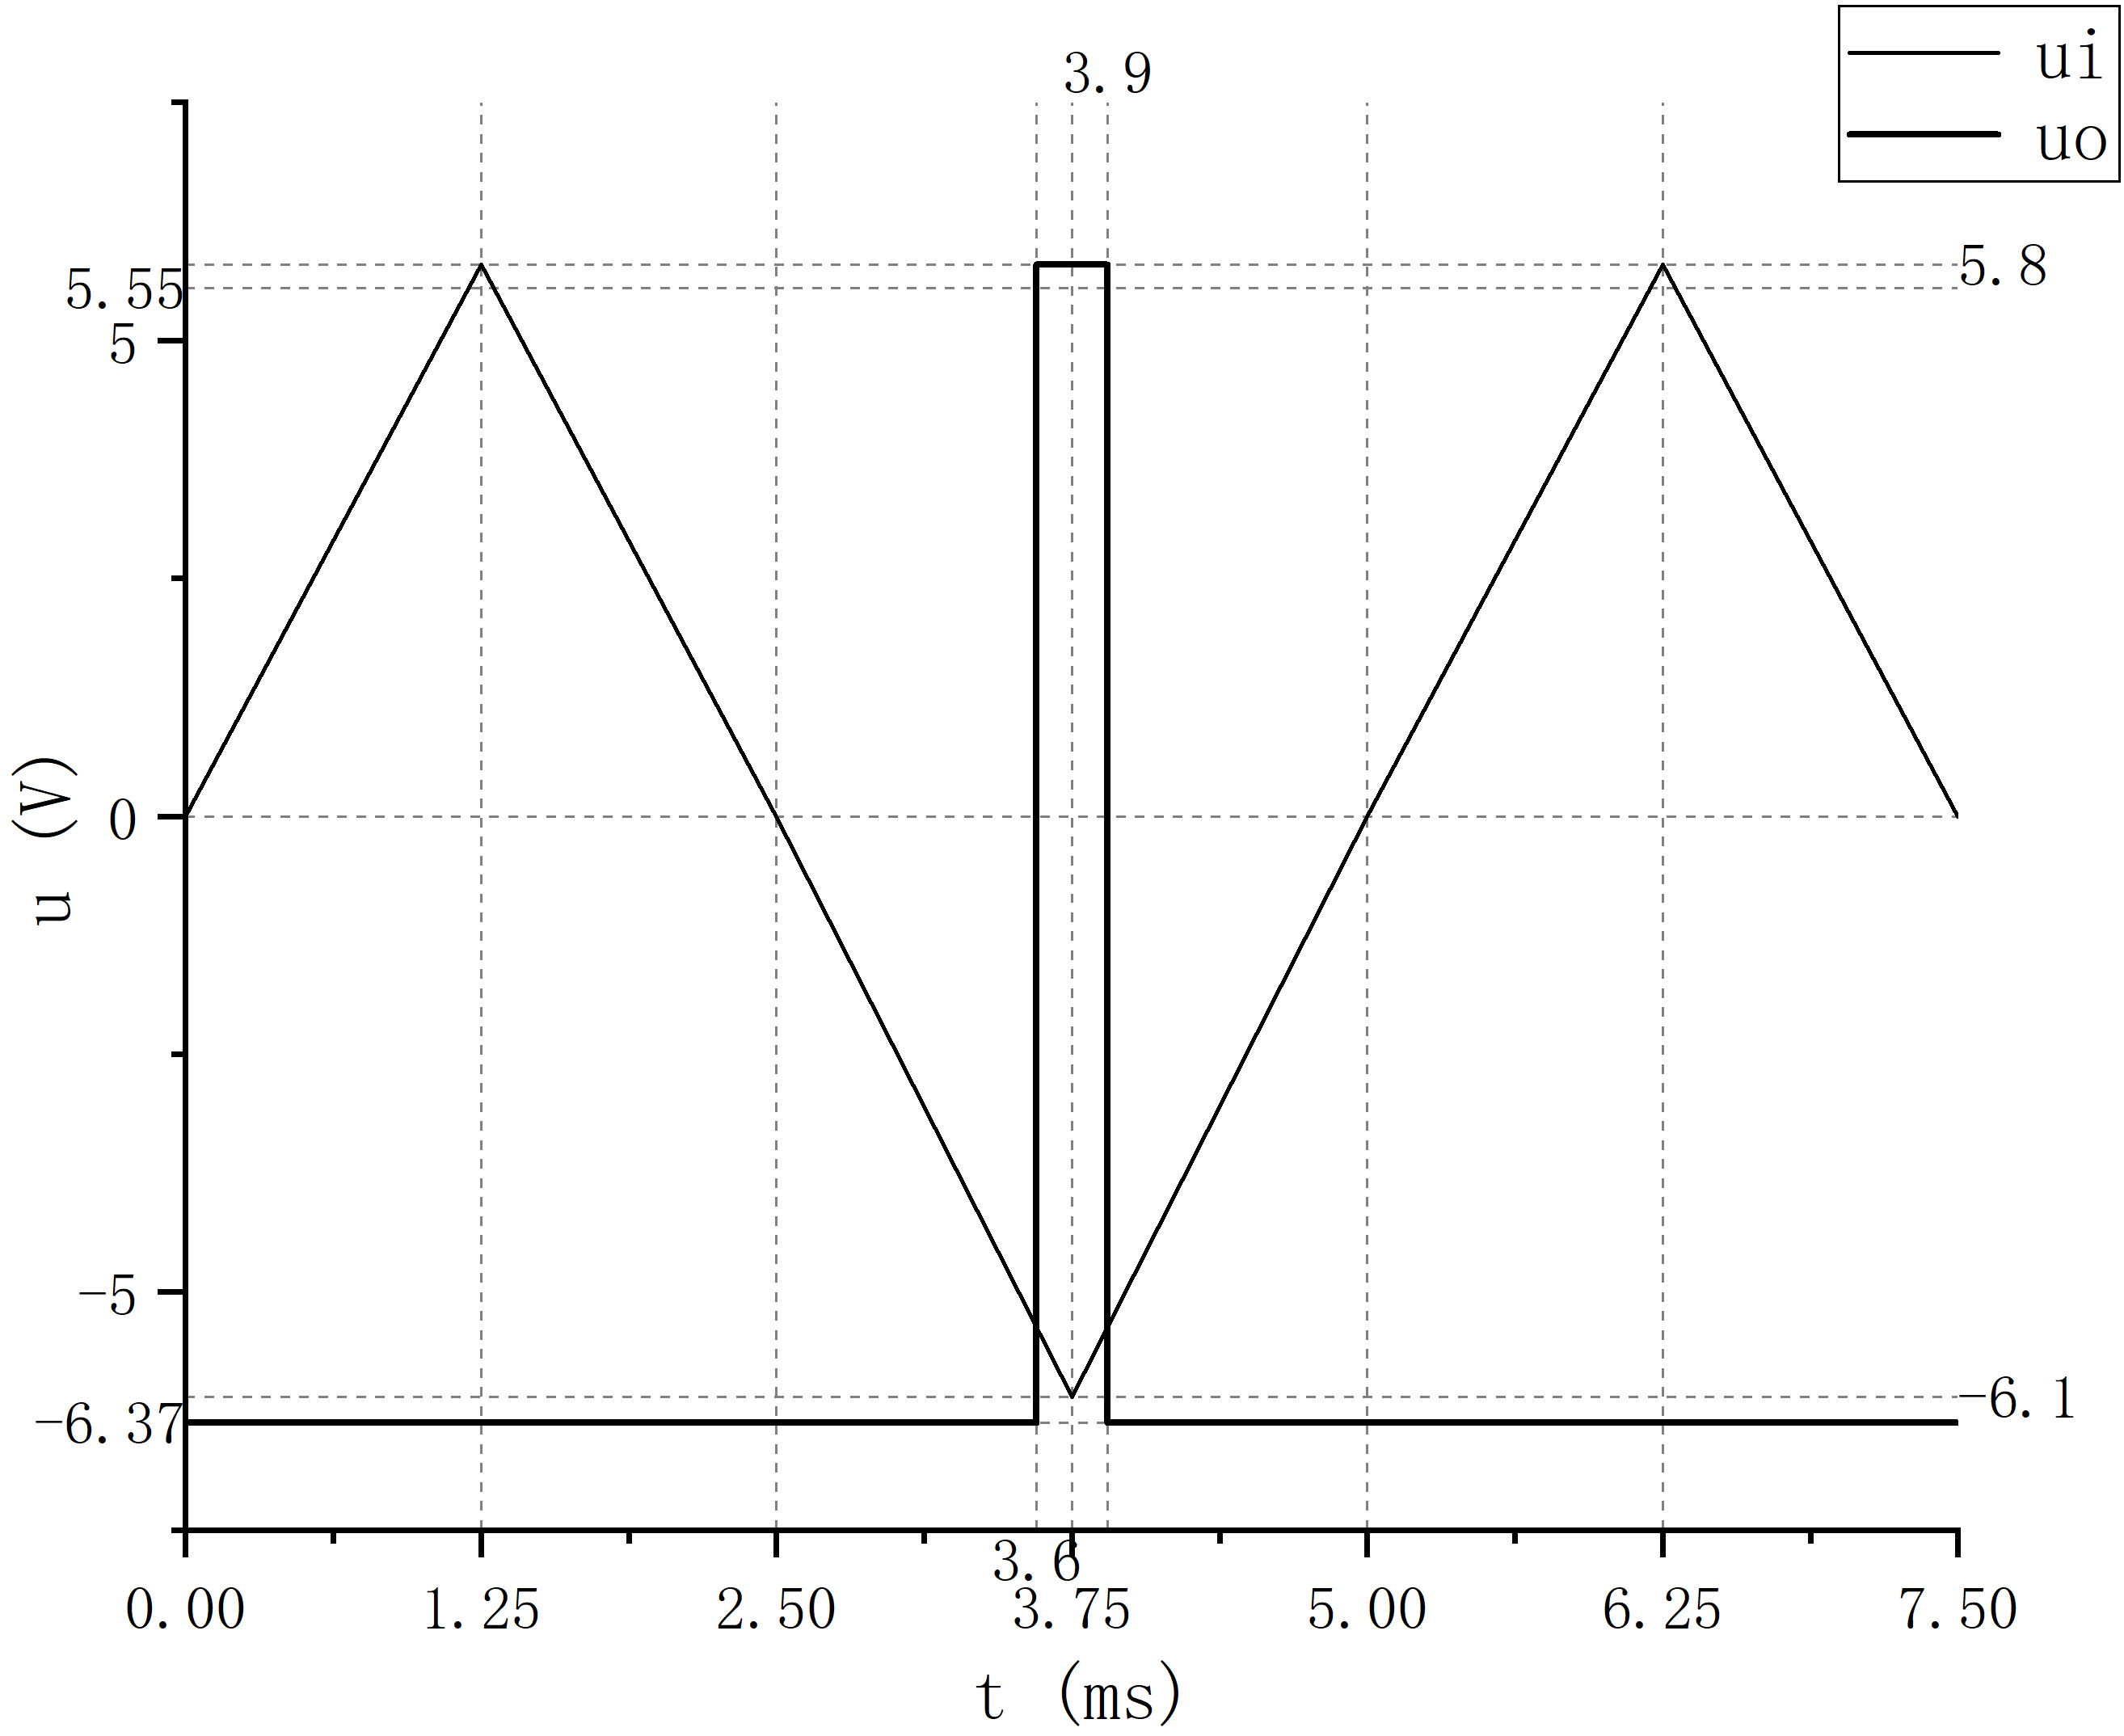
\includegraphics[width=8cm]{1-3-1}
	 \caption{实验一输入输出波形, $U_{REF}=-5\mr{V}$}
	 \label{fig:1-3-1}
	 \end{figure}
	 \begin{figure}[H]
	 	\centering
	 	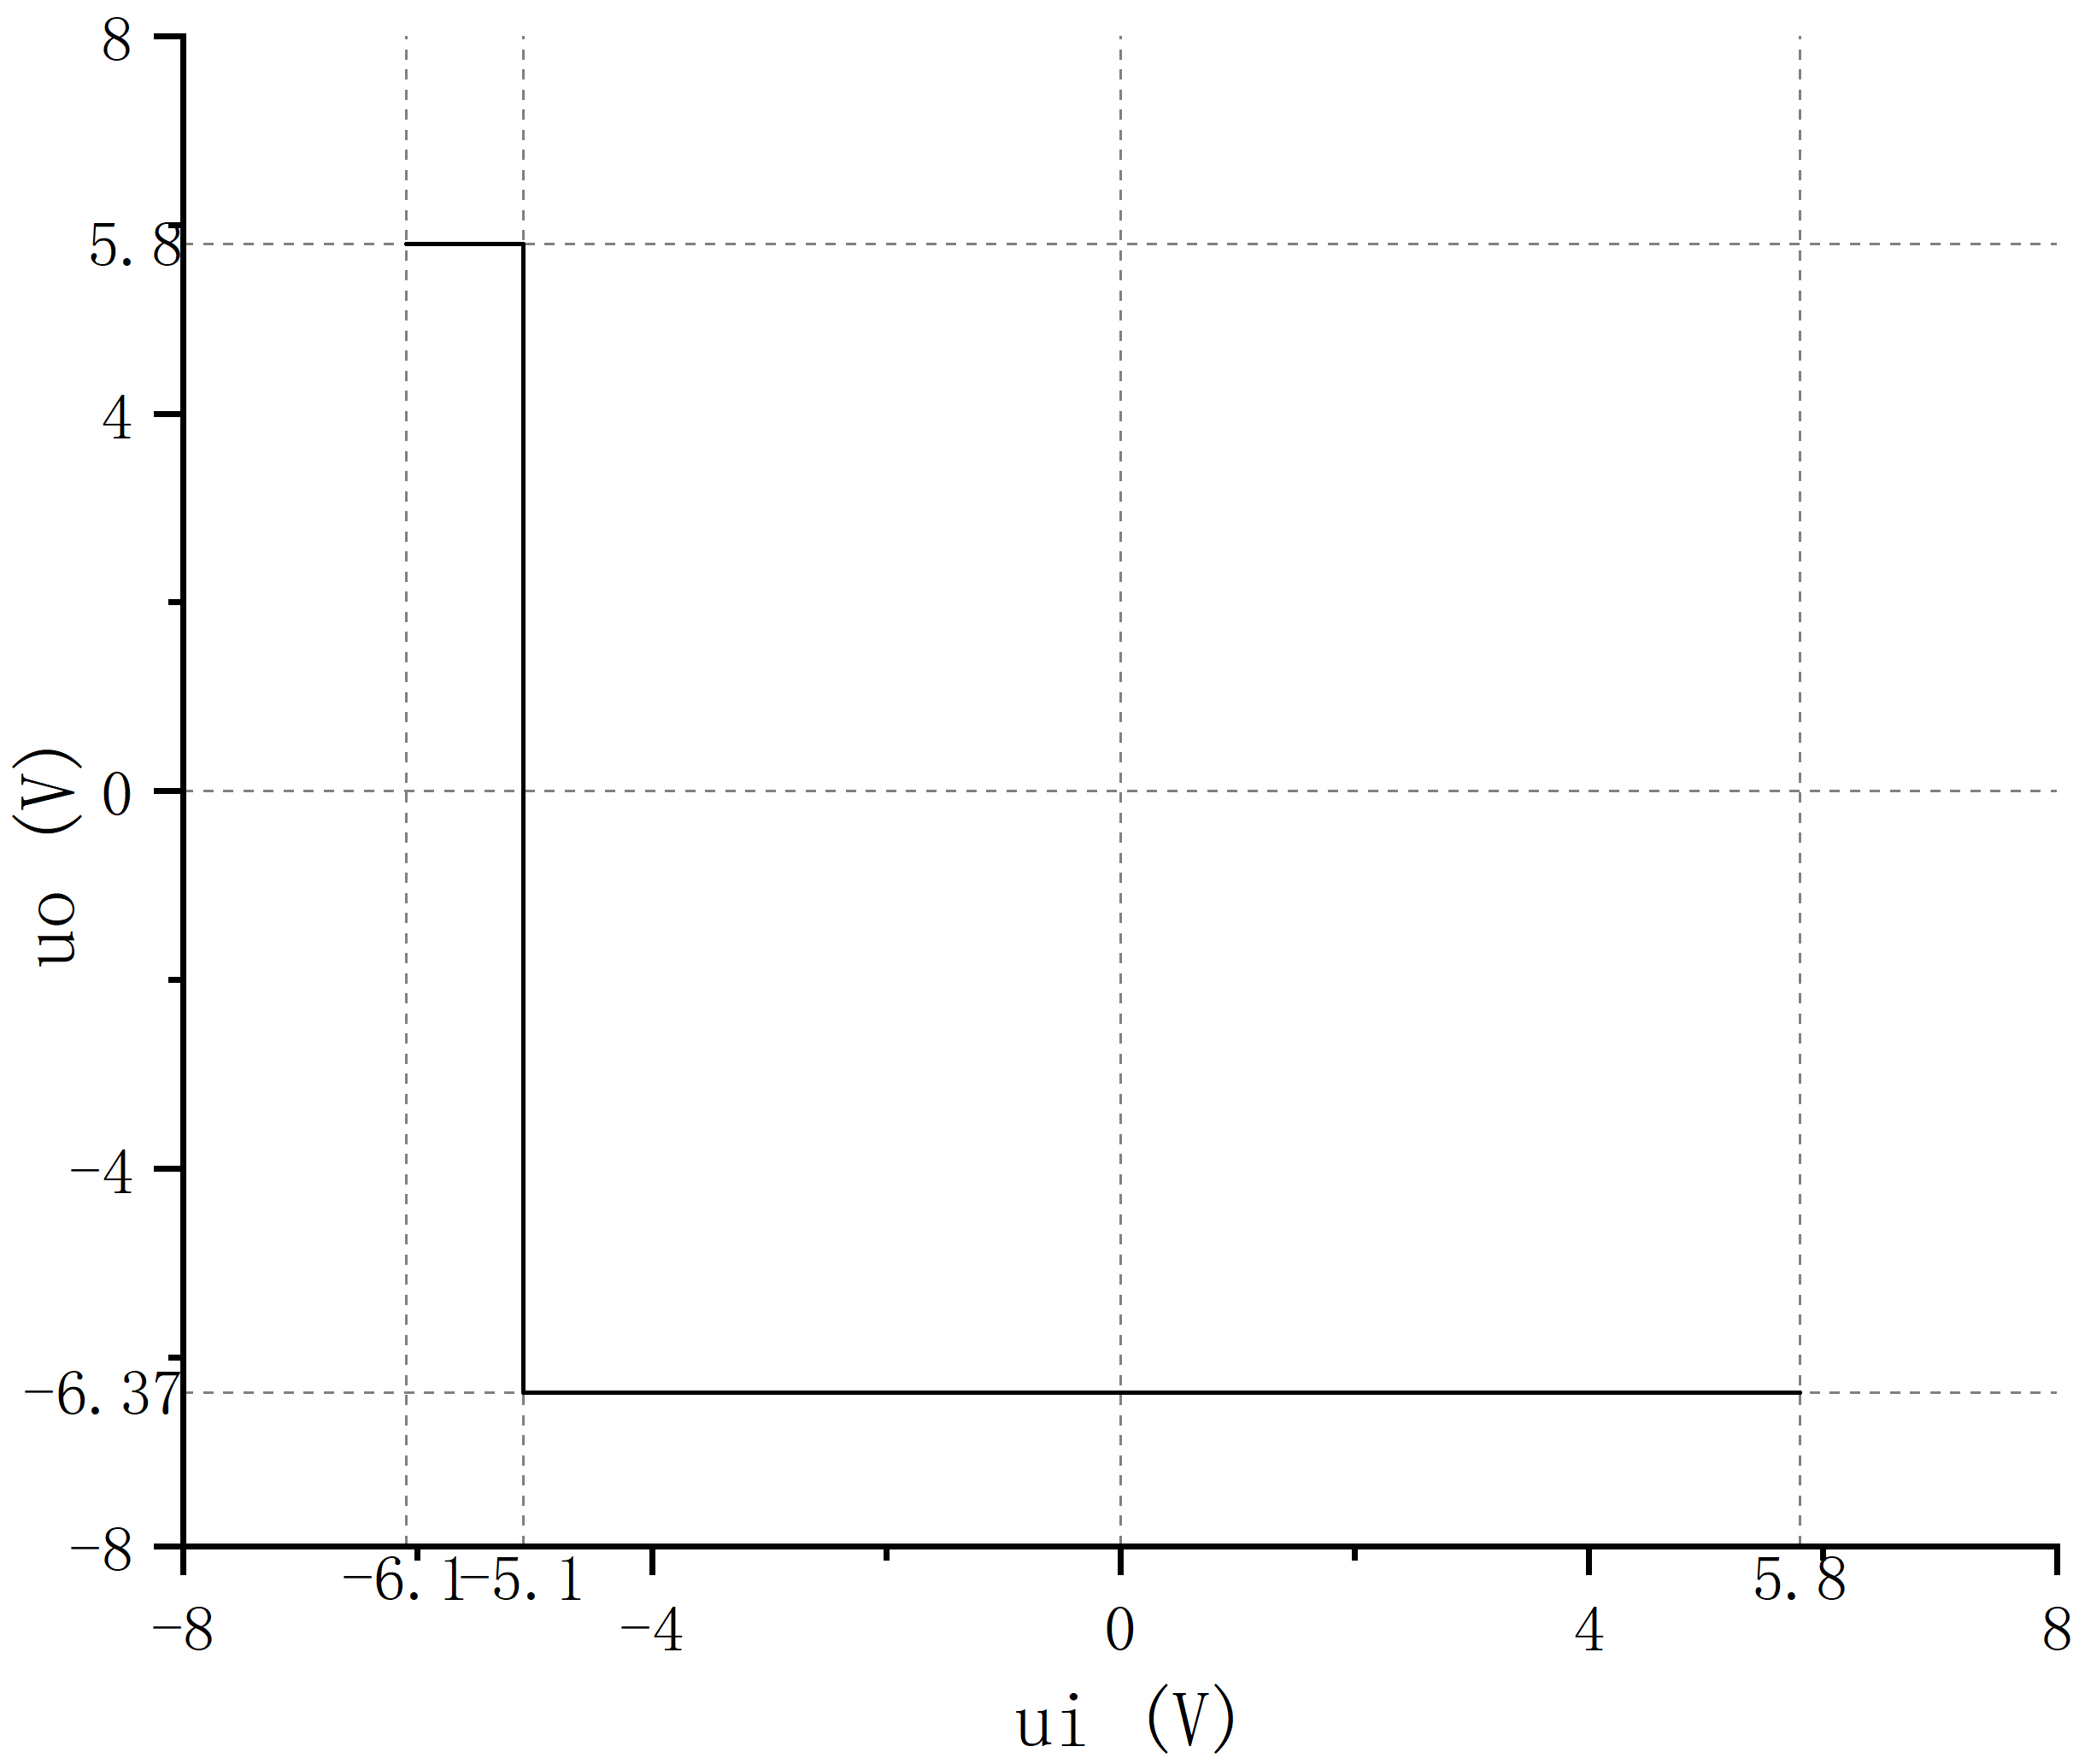
\includegraphics[width=8cm]{1-3-2}
		 \caption{实验一传输特性曲线, $U_{REF}=-5\mr{V}$}
		 \label{fig:1-3-2}
	 \end{figure}
		\end{itemize}
	\subsubsection{实验分析}
		根据理论,若 $u_i>U_{REF}$ ,那么输出高电平,反之输出低电平。实验得到的门限电压与 $U_{REF}$ 吻合得比较好。
		\par 输入波形和输出波形的周期是一样的,都是 $5\mr{ms}$。
		\par 门限电压附近的李萨如图形比较模糊,若进一步放大,发现门限电压其实是由两个更精细的电压组成的,间隔大约几百 mV 。
		\par 高低电平的值误差比较大。理论值应该是 $\pm6\mr{V}$ ,但实际上为 $6.3\mr{V},~-5.8\mr{V}$ 左右,这个误差可能有如下来源:
		\begin{itemize}
		 \item 双向稳压管的两个方向特性不对称。
		 \item 运算放大器的正负电压特性不对称。
		 \item 经过多次实验,发现示波器的高值和低值总是不能做到对称(会比峰值高/低零点几V),所以可能示波器也有误差。
		\end{itemize}

\subsection{实验二:窗口比较器}
	\subsubsection{实验数据}
		测量值:$R=10.007\mr{k}\Omega$。
		\begin{figure}[H]
		 \centering
		 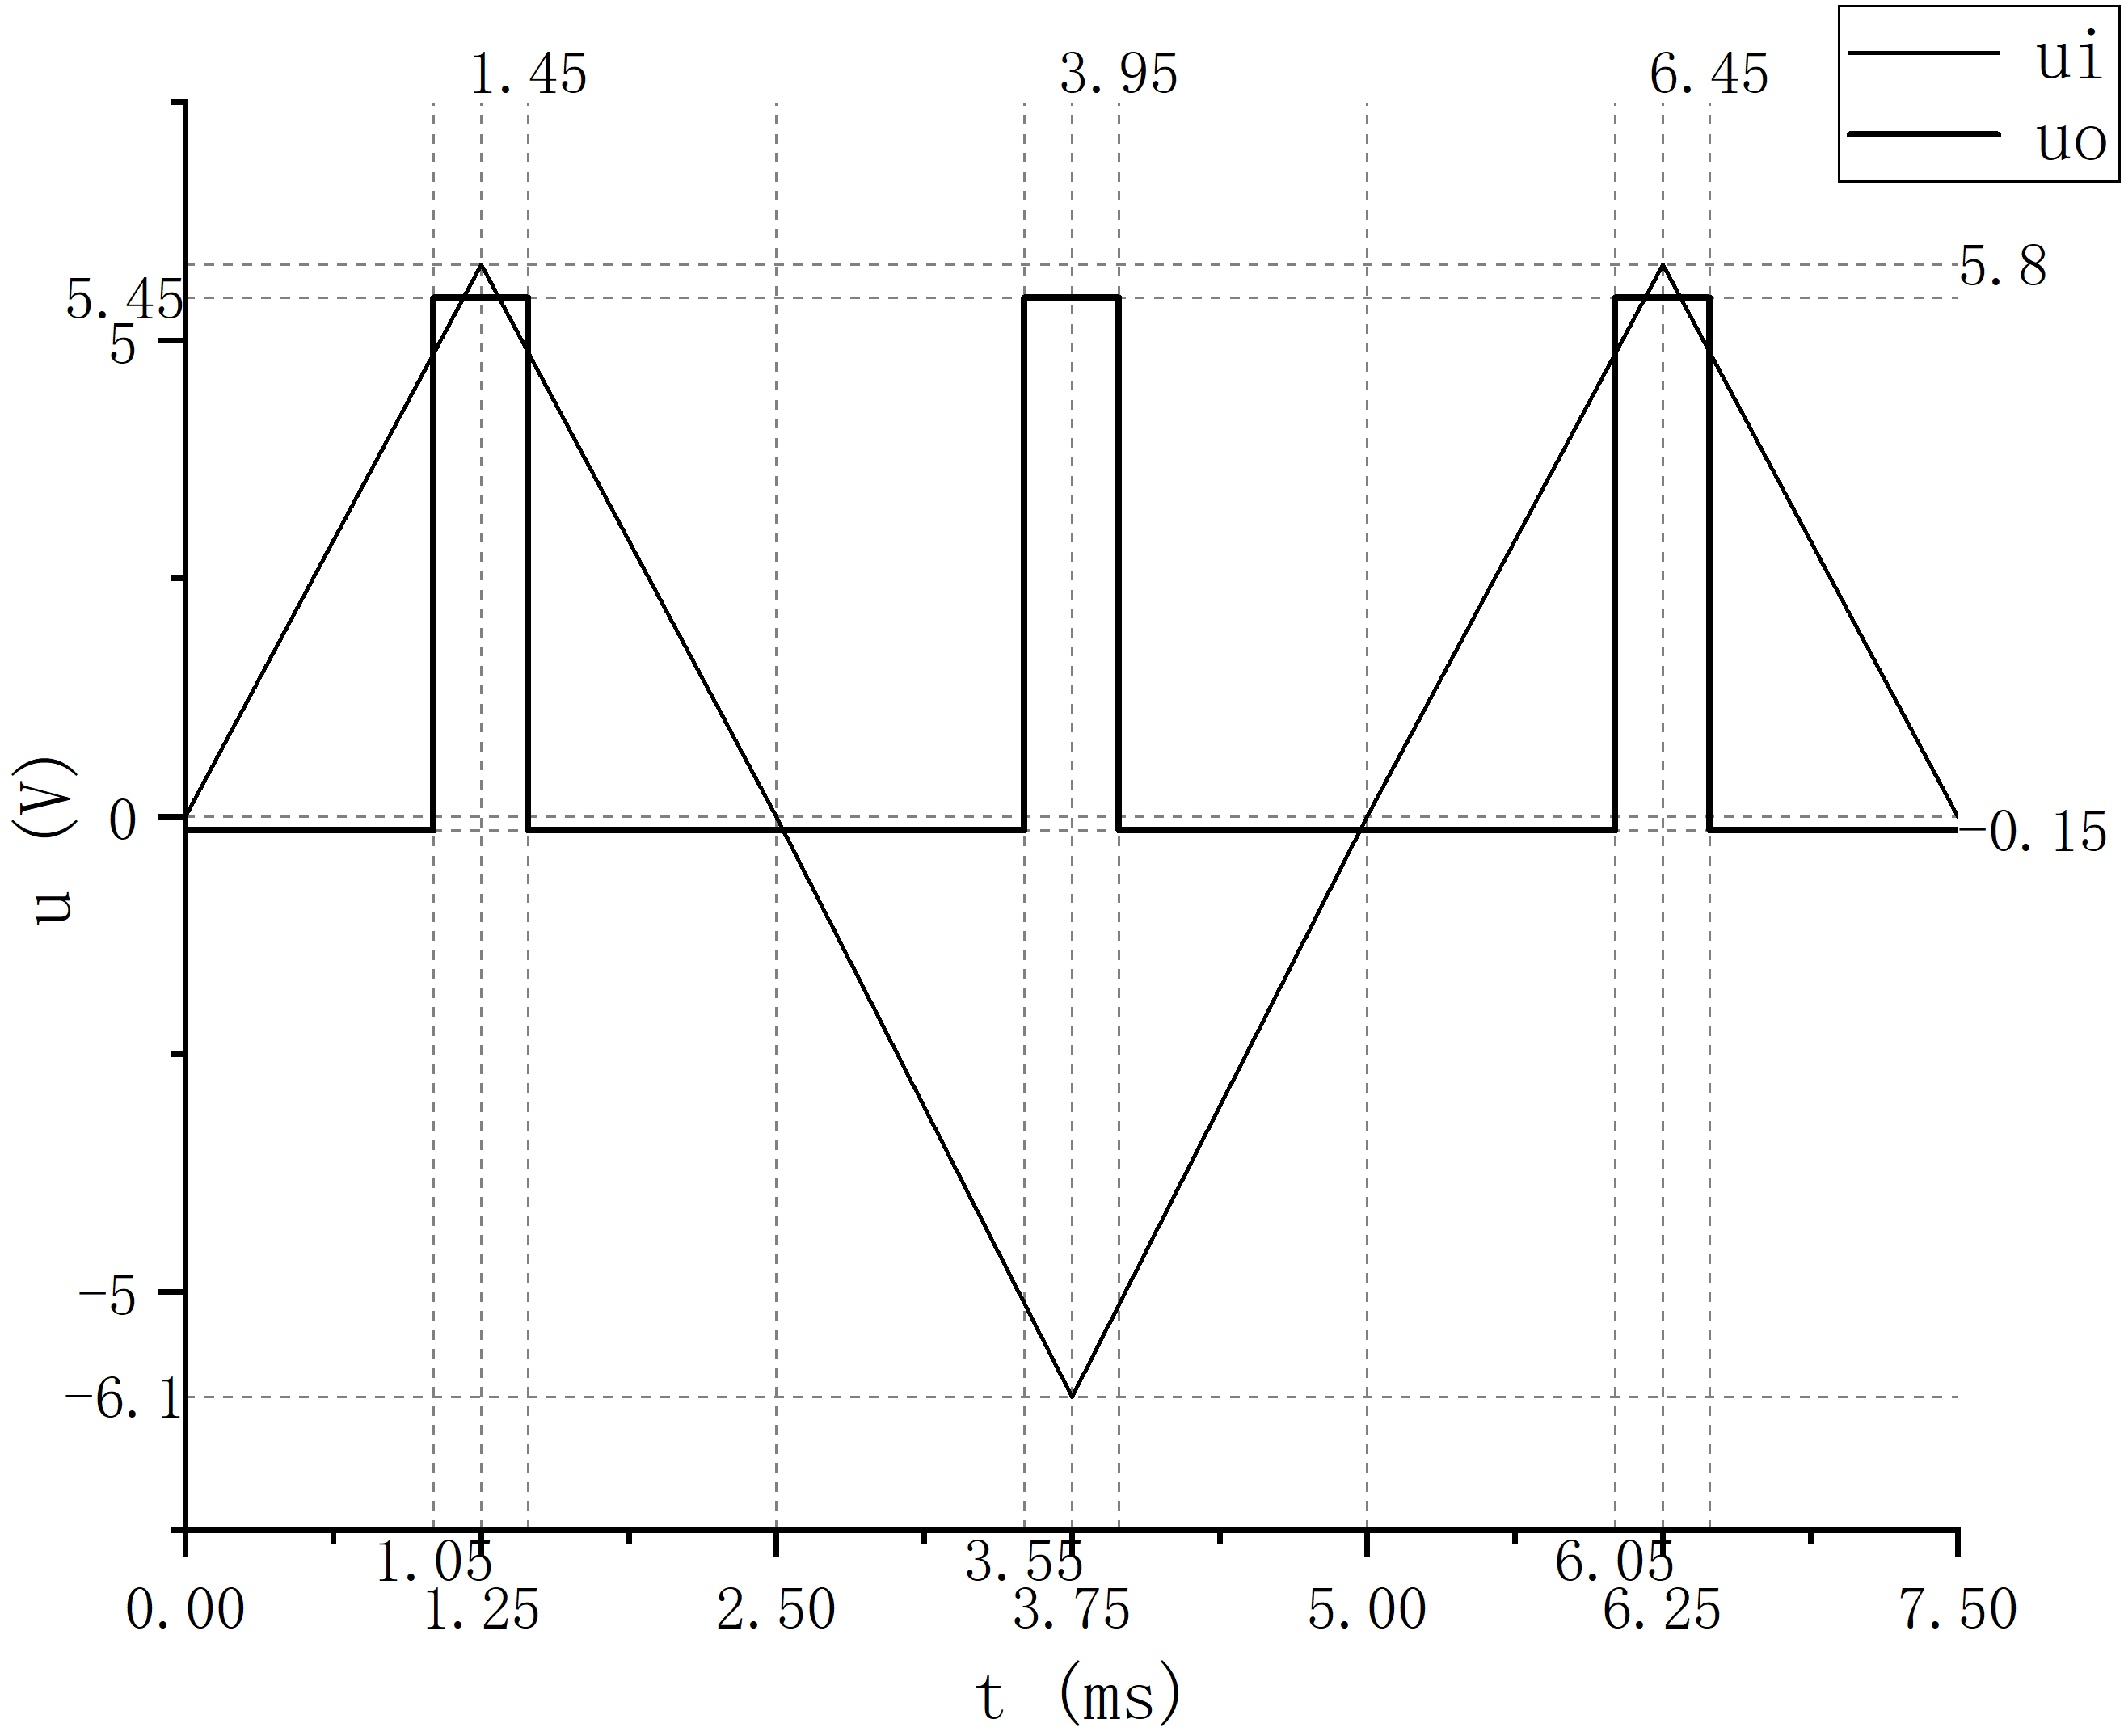
\includegraphics[width=8cm]{2-1}
		 \caption{实验二的输入输出波形}
		 \label{fig:2-1}
		\end{figure}
		\begin{figure}[H]
		 \centering
		 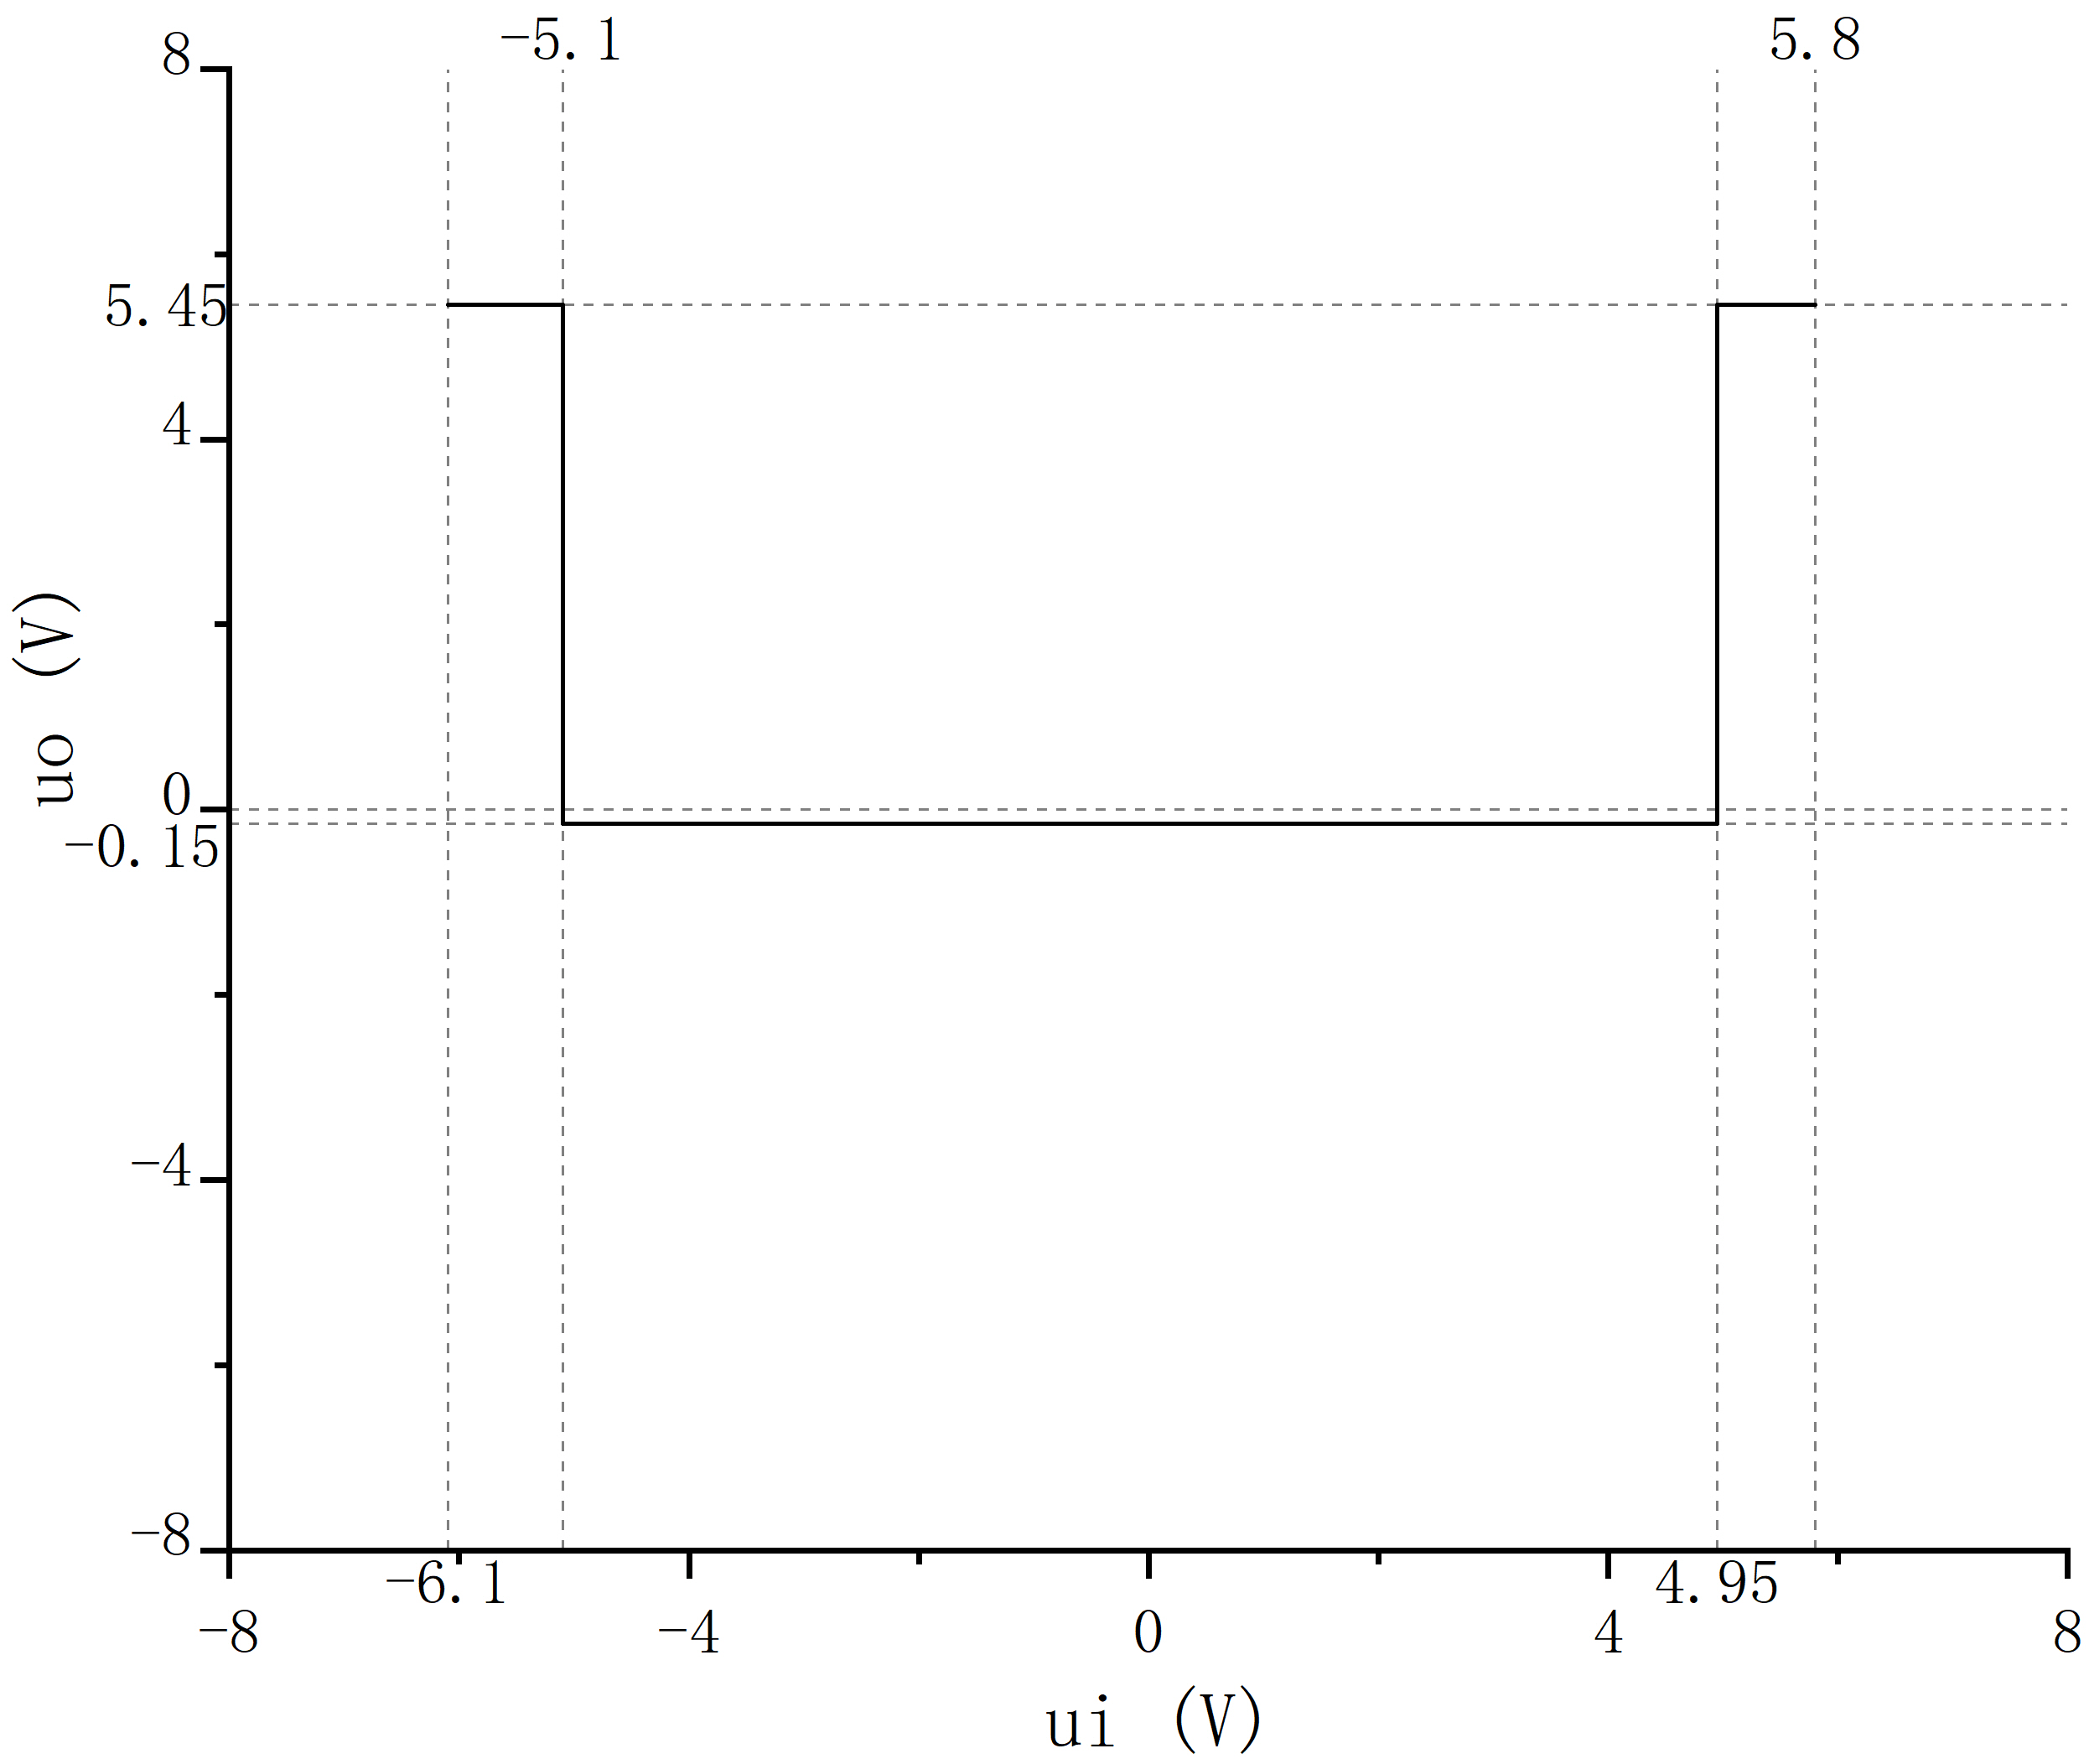
\includegraphics[width=8cm]{2-2}
		 \caption{实验二的传输特性曲线}
		 \label{fig:2-2}
		\end{figure}
	\subsubsection{实验分析}
		实验有高低两个门限电压,低于低门限电压或高于高门限电压都会输出高电平,反之输出0电平。高低门限电压与理论值 $\pm6\mr{V}$ 比较接近。
		\par 输入波形的周期是 $5\mr{ms}$ ,但输出波形的周期减半,为 $2.5\mr{ms}$ ,理由是:因为输入电平太高或太低都能输出高电平,所以在一个输入信号周期内,可以输出两段高电平。
		\par 门限电压附近的李萨如图形比较模糊,若进一步放大,发现门限电压其实是由两个更精细的电压组成的,间隔大约几百 mV 。
		\par 类似地,实验结果得到的输出高电平依然偏小。关于这个误差的解释同实验一。
\subsection{实验三:滞回比较器}
	\subsubsection{实验数据}
		测量值:$R_f=10.116\mr{k}\Omega,~R=10.007\mr{k}\Omega$。
		\begin{figure}[H]
		 \centering
		 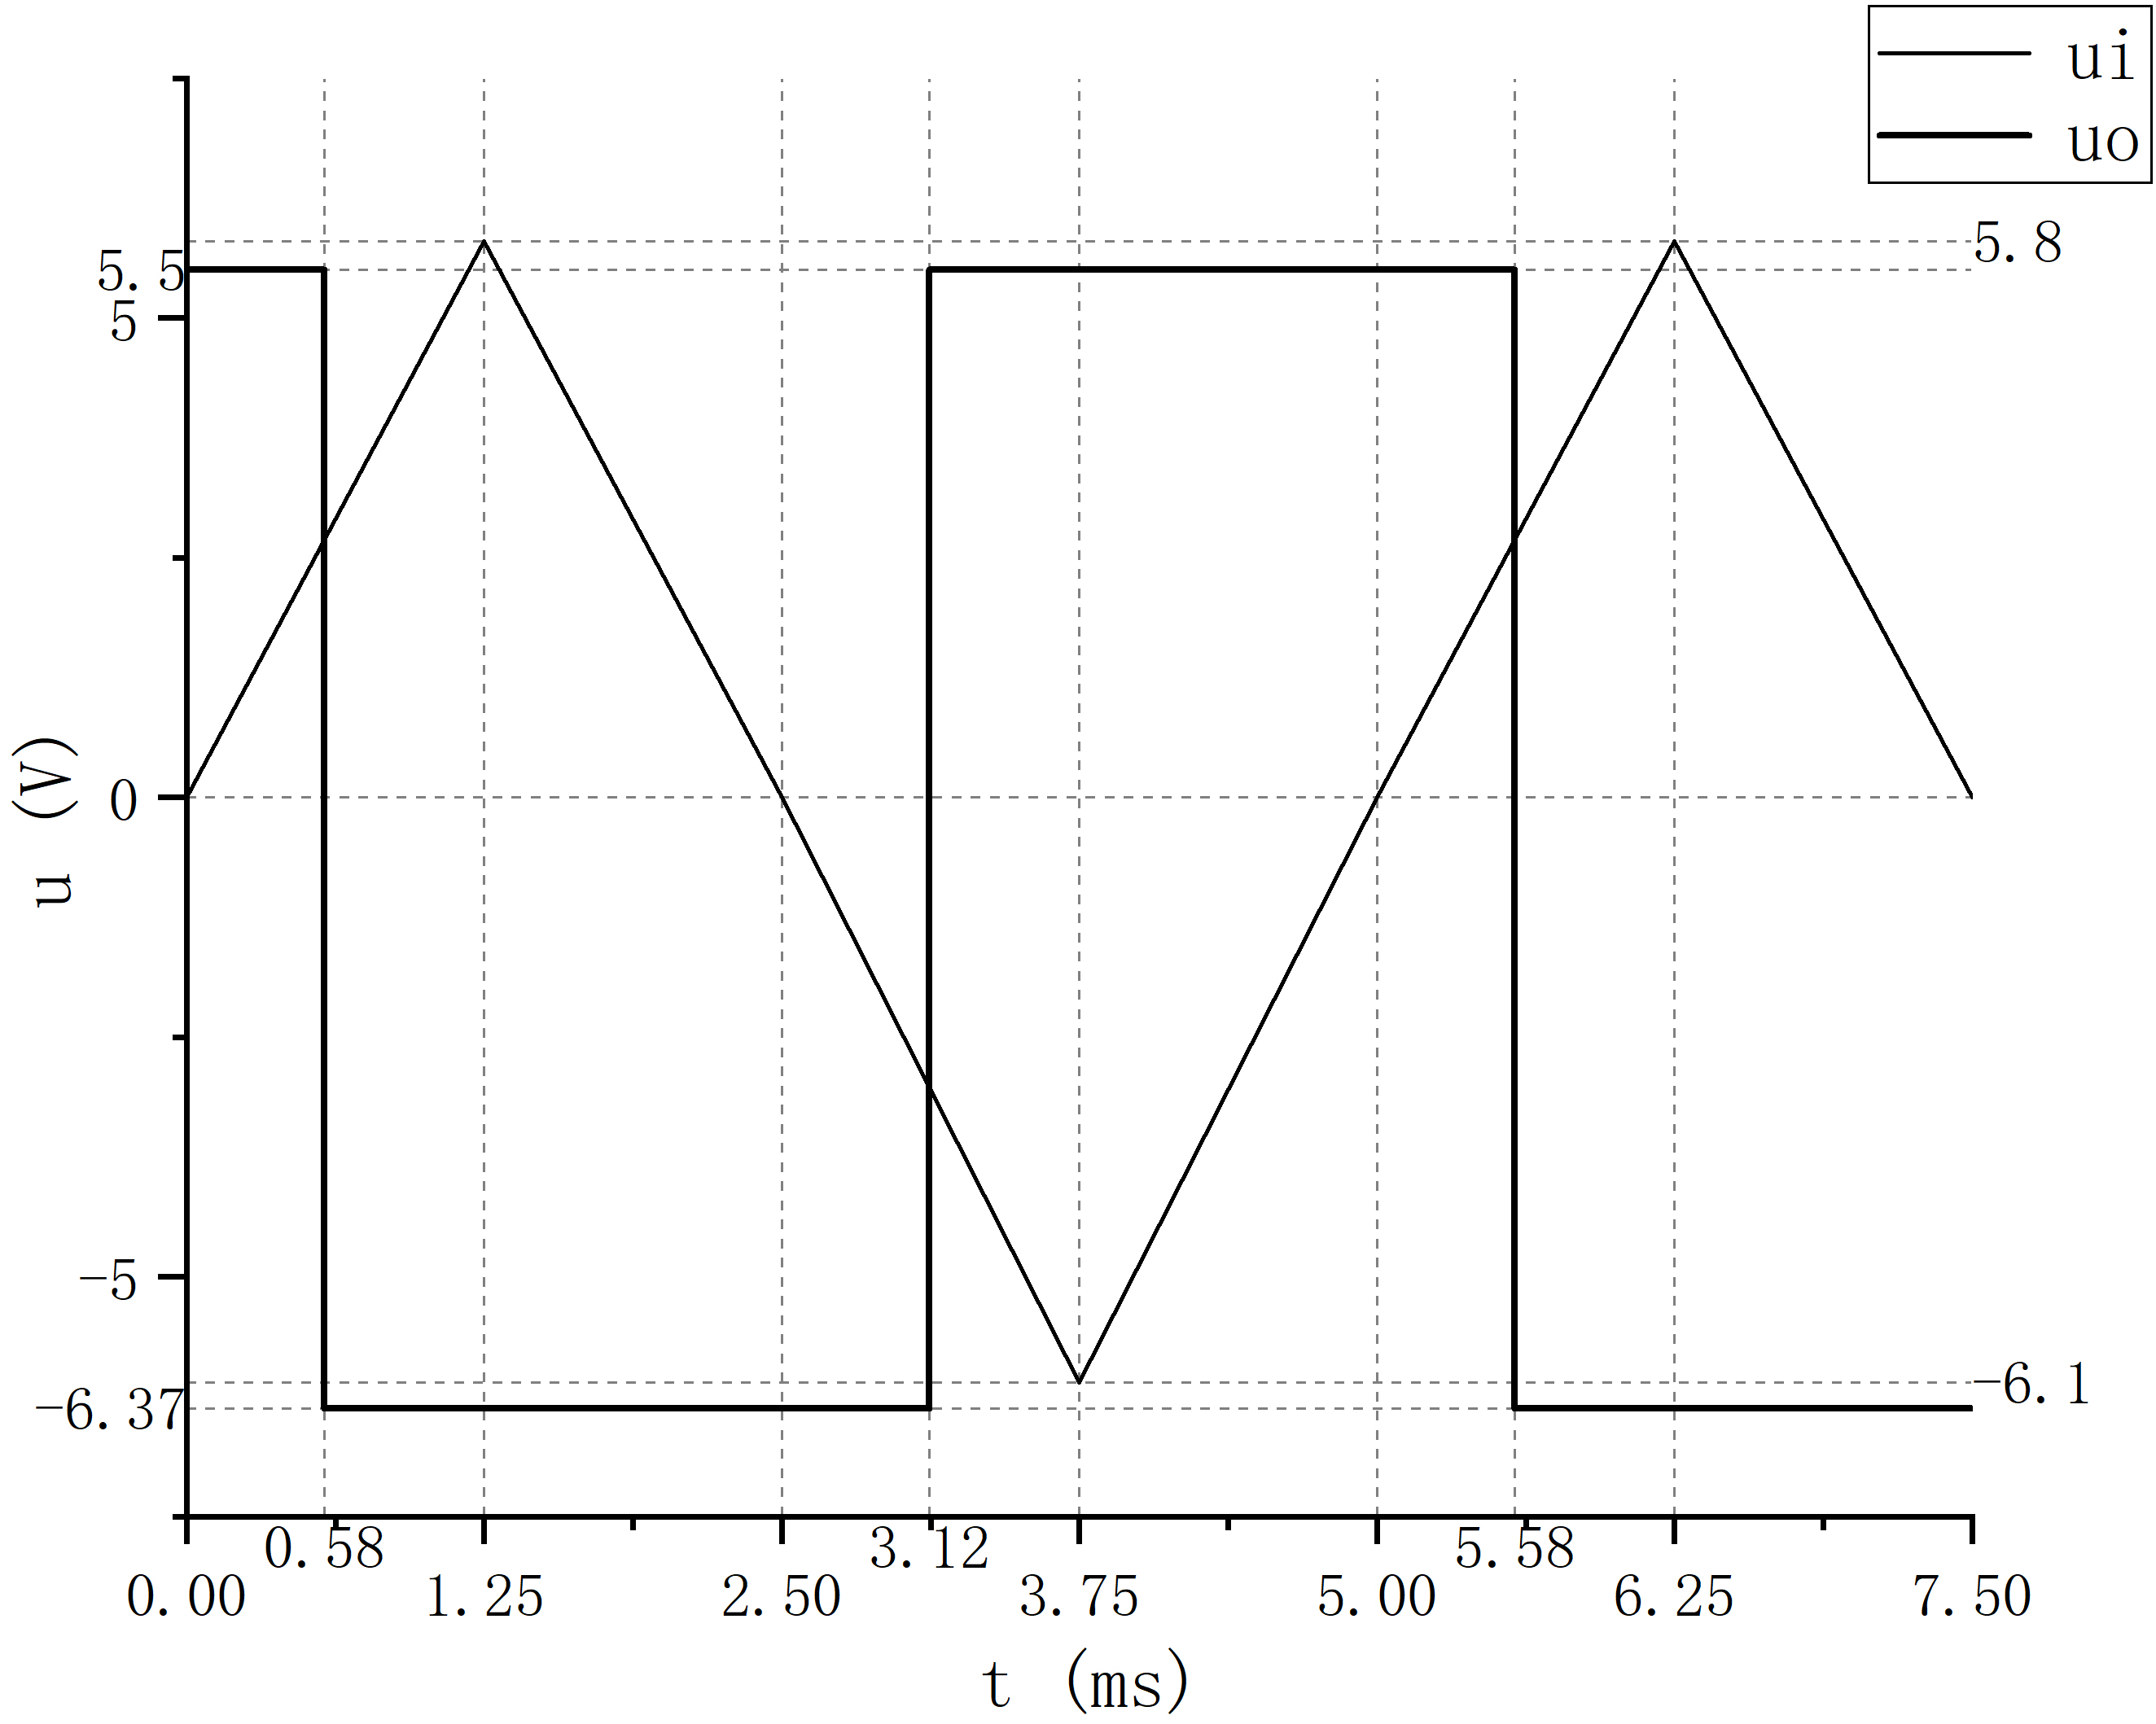
\includegraphics[width=8cm]{3-1}
		 \caption{实验三的输入输出波形}
		 \label{fig:3-1}
		\end{figure}
		\begin{figure}[H]
		 \centering
		 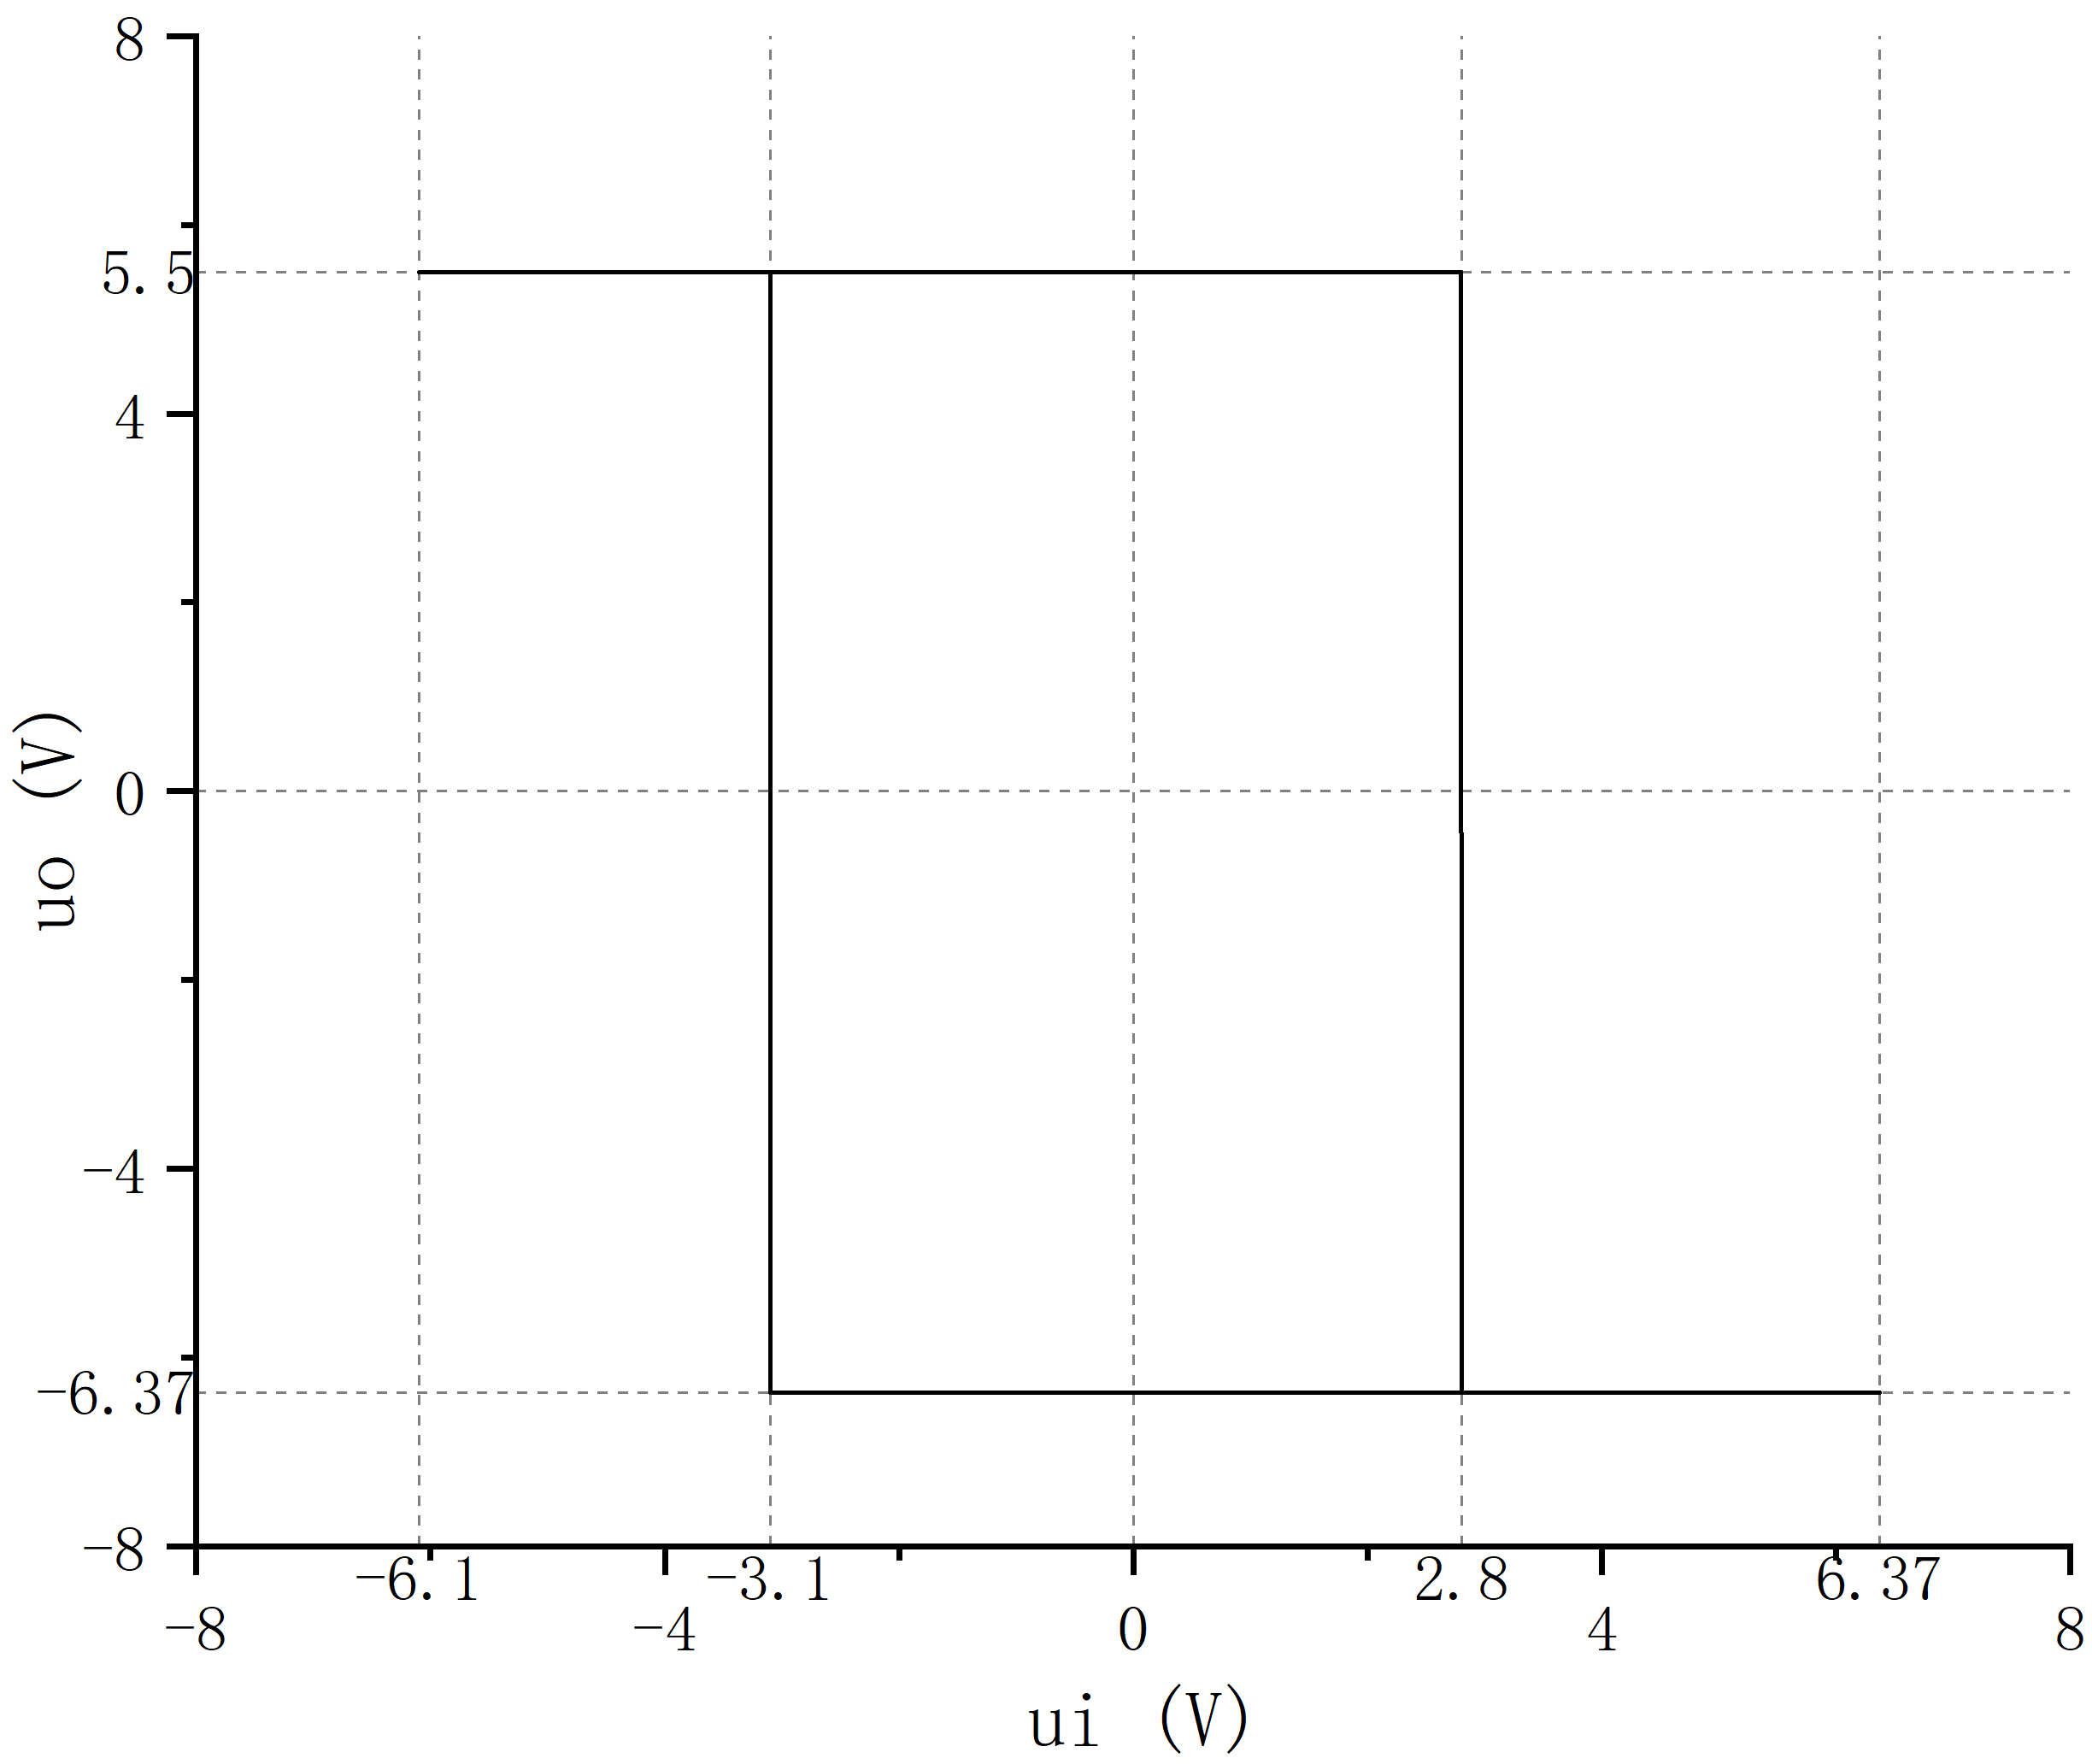
\includegraphics[width=8cm]{3-2}
		 \caption{实验三的传输特性曲线}
		 \label{fig:3-2}
		\end{figure}
	\subsubsection{实验分析}
		可以看到,输出信号(方波)与输入信号(三角波)的交点电平是不一样的。以 $t=3.12\mr{ms}$ (记为 $t_1$ ) 和 $t=5.58\mr{ms}$ (记为 $t_2$ ) 为例,因为 $t_1$ 附近输入电平是在变低的,所以门限电压是较低的 $-3.1\mr{V}$ ;在 $t_2$ 附近输入电平是在变高的,所以门限电压是较高的 $2.8\mr{V}$ 。
		\par 由此修改传输特性曲线,以看出这种滞回效应:
		\begin{figure}[H]
		 \centering
		 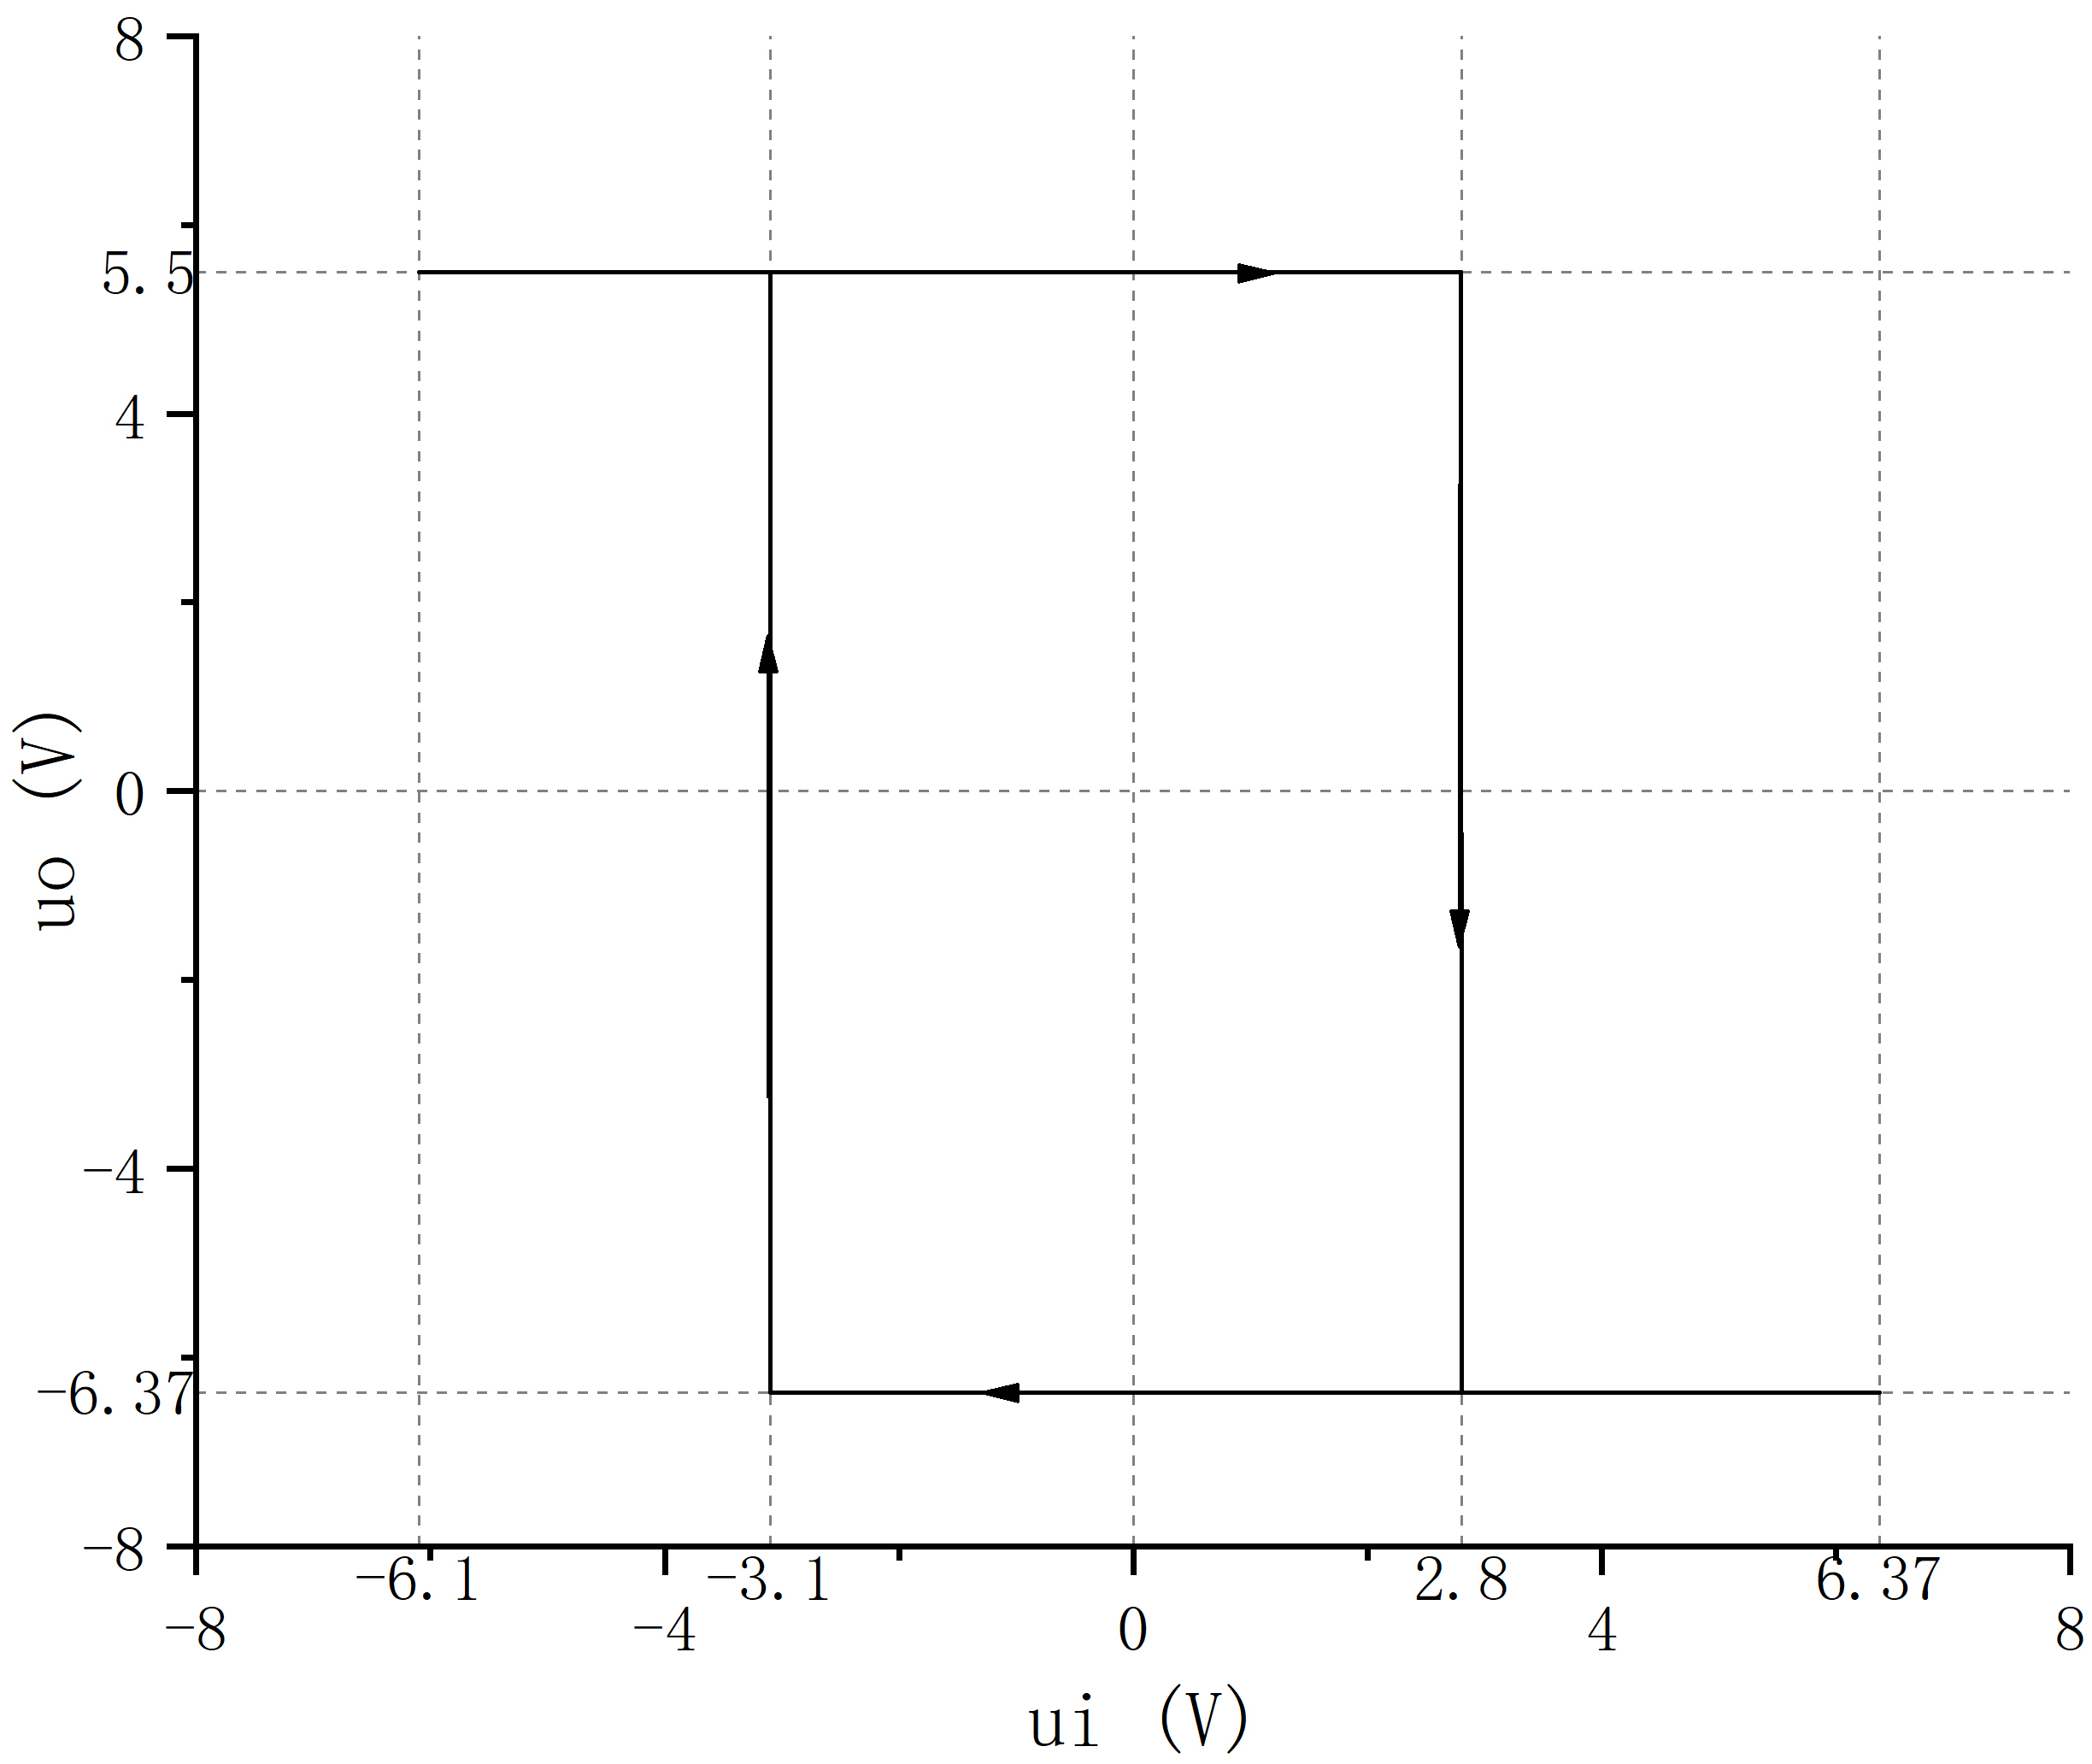
\includegraphics[width=8cm]{3-2-edited}
		 \caption{实验三的滞回传输特性曲线}
		 \label{fig:3-2-e}
		\end{figure}
		\par 由实际数据计算 $U_{T\pm}$:
		\[ U_{T+}=\frac{R}{R+R+R_f}U_{om+}=2.735\mr{V} \]
		\[ U_{T-}=\frac{R}{R+R_f}U_{om-}=-3.168\mr{V} \]
		而实际值为 $U_{T+}=2.8\mr{V},~U_{T-}=-3,1\mr{V}$ ,吻合得比较好。
		\par 由此可见,滞回比较器的电路并没有增添许多额外误差。之所以门限电压偏离理论值 $\pm3\mr{V}$ ,是因为 $U_{om\pm}$ 偏离了理论值。而 $U_{om\pm}$ 产生较大误差的原因,同实验一。
\subsection{实验四:方波发生器(振荡器)}
	\subsubsection{实验数据}
		测量数据:$R=10.007\mr{k}\Omega,~R_F=10.116\mr{k}\Omega,~R_F=23.74\mr{k}\Omega,~C=0.0112\upmu\mr{F},~f=1.66\mr{kHz}$。
		\begin{figure}[H]
		 \centering
		 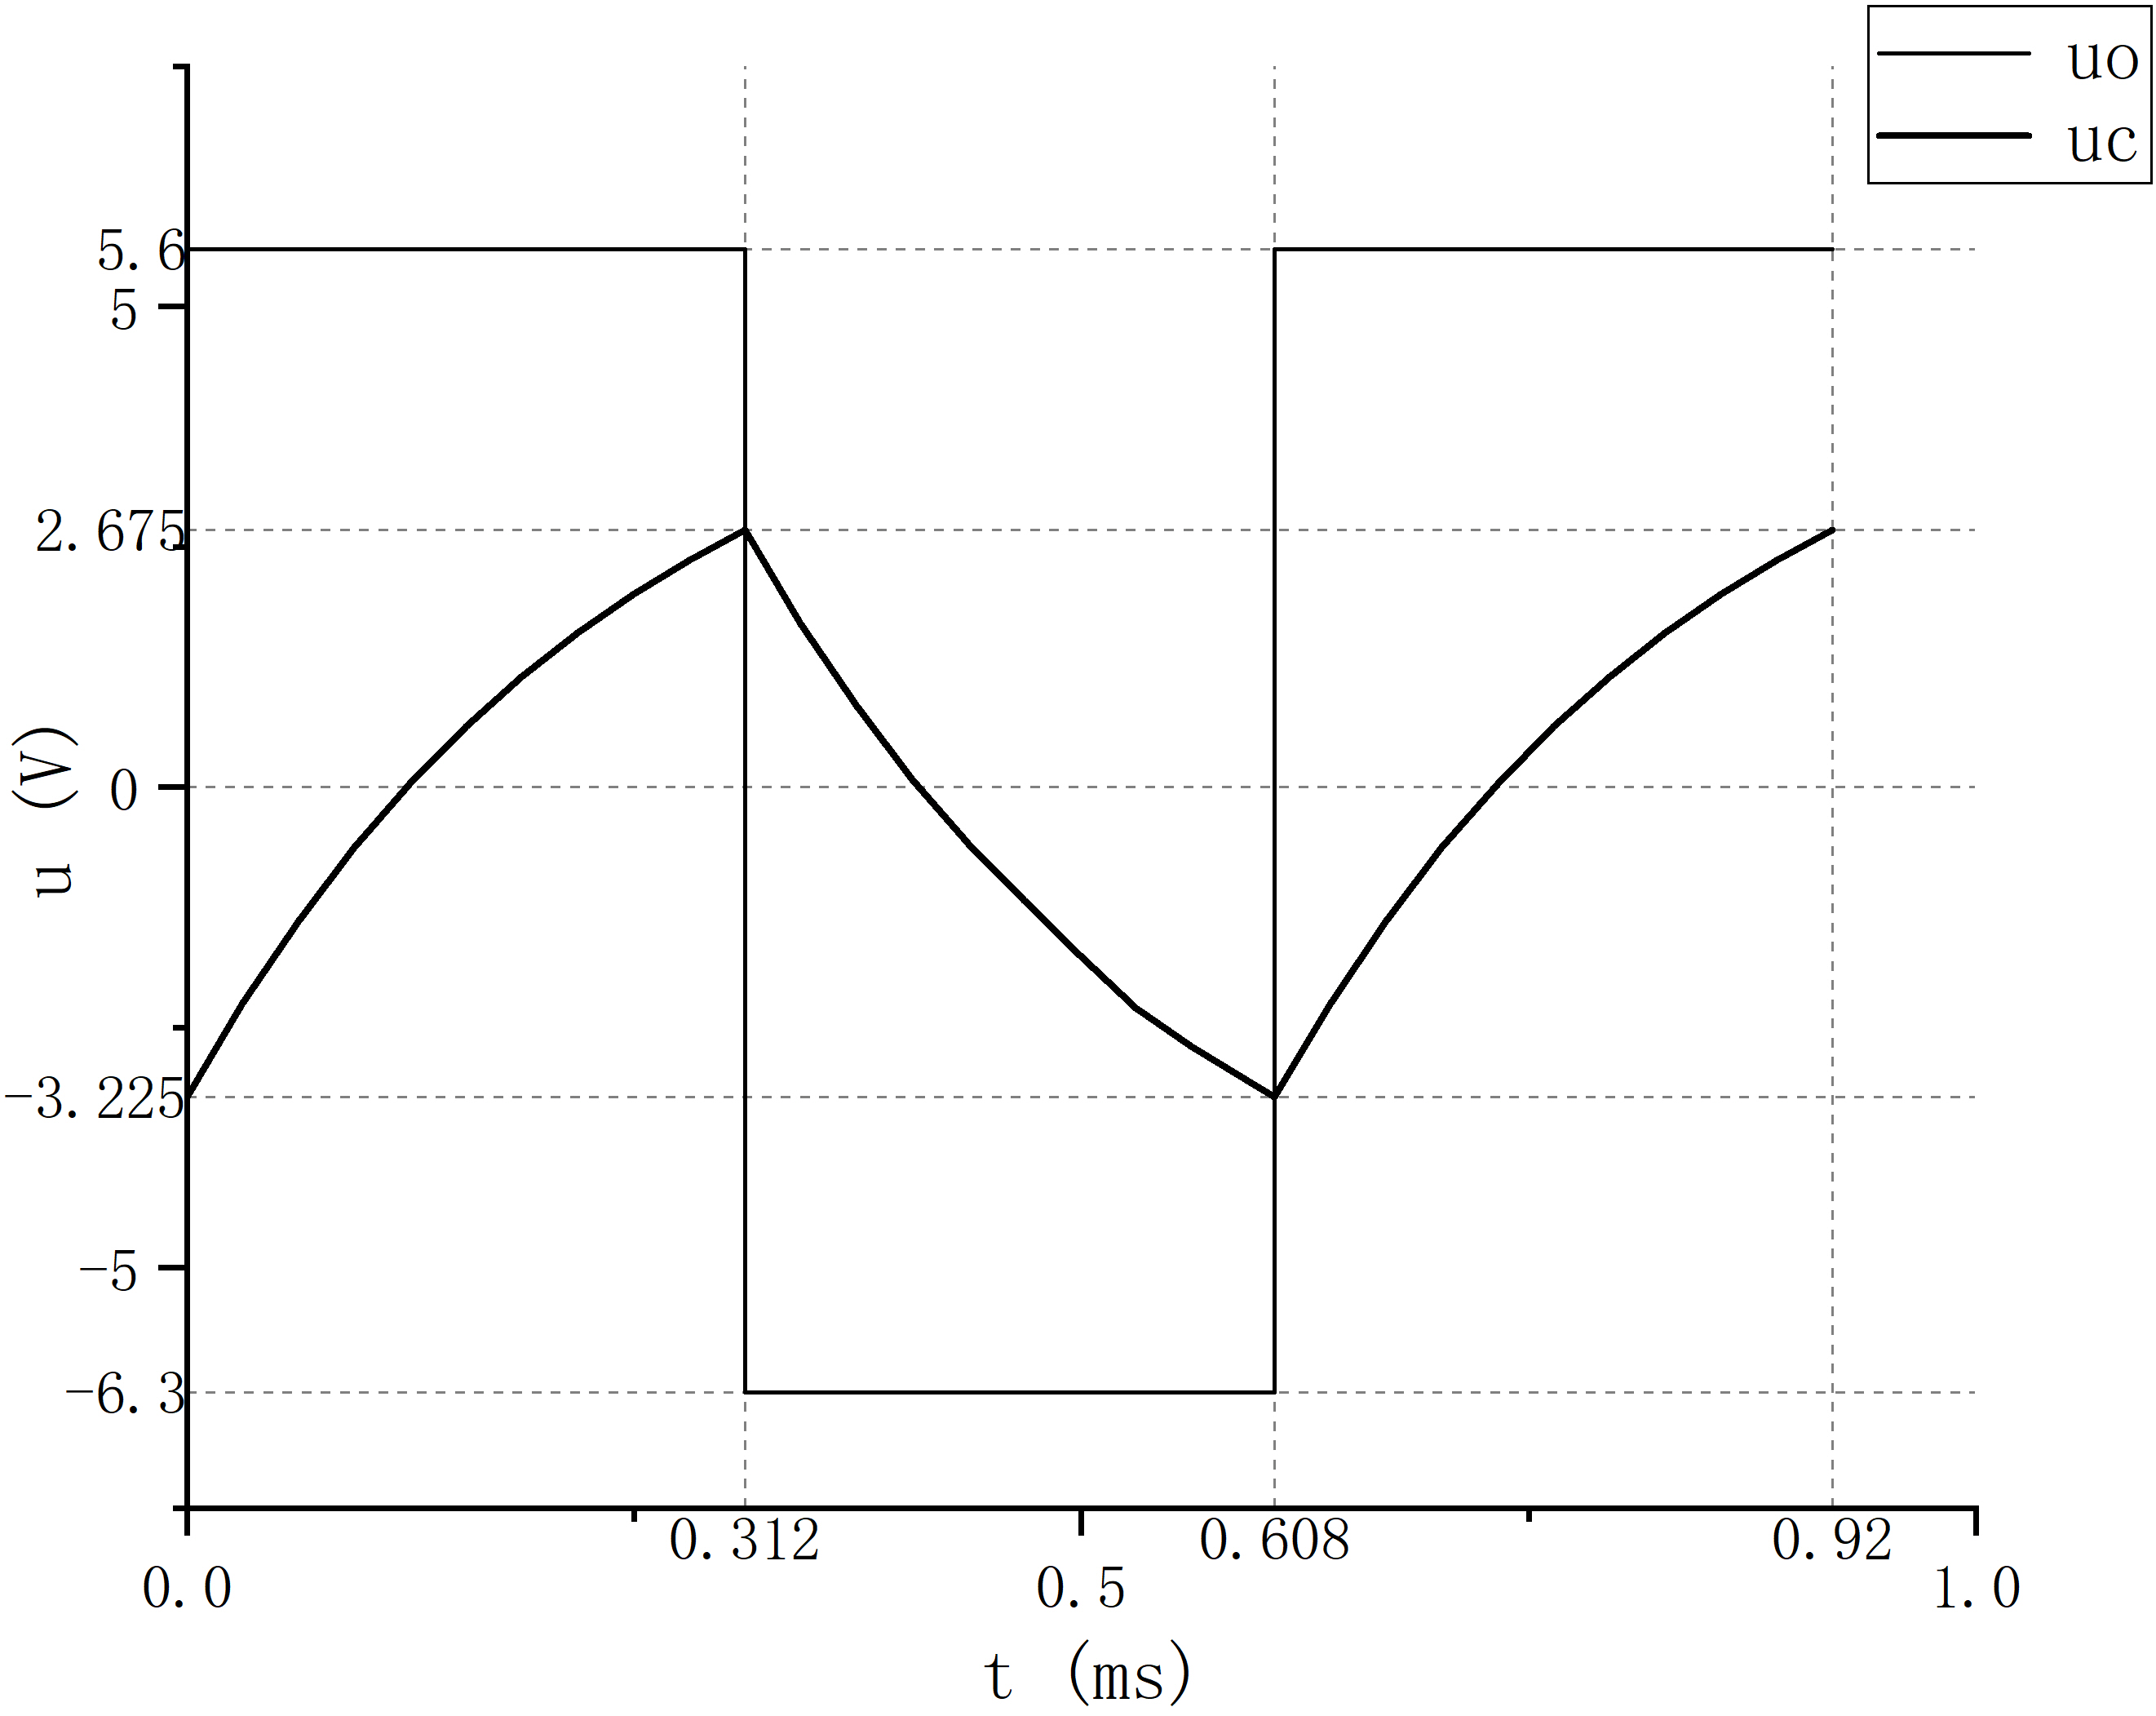
\includegraphics[width=8cm]{4}
		 \caption{实验四的输入输出波形曲线}
		 \label{fig:4}
		\end{figure}
	\subsubsection{实验分析}
		时间常数 $\tau=R_FC=0.266\mr{ms}$。如果 $u_o$ 不是方波而是恒为 $5.6\mr{V}$ ,那么指数曲线在无穷时间处必趋向于 $5.6\mr{V}$ 。又因为 0 时刻的 $u_C=-3.225\mr{V}$ ,由此写出第一段指数曲线的表达式:
		\[ u_C(t)=5.6-8.825\exp{\left(-\frac{t}{0.2659\mr{ms}}\right)}\,\mr{V},~0<t<0.312\mr{ms} \]
		代入 $t=0.312\mr{ms}$ ,得到:
		\[ u_C(0.312\mr{ms})=2.870\mr{V} \]
		实际值为 $2.675\mr{V}$ 。考虑到这是一个简单的近似计算,其精度尚可。所以我们得到的 $u_C$ 图像误差应该不会很大。
		\par 方波的高低峰值偏低,其理由同样参实验一。
\section{实验总结}
理想运算放大器是处于深度反馈状态的,其两输入端口电压必定一致。但是实际运放总存在一个非线性区,在非线性区,运放输出电压饱和,几乎为定值。借用这一特性,可以用特殊种类的运算放大器构建电压比较电路,可以实现诸多功能,譬如:
\begin{enumerate}
 \item 与一门限比较(单限比较器)。
 \item 与两个门限电压比较(窗口比较器)。
 \item 在电压变化方向不同时,门限电压也不同(滞回比较器)。
 \item 让运算放大器自振荡,从而产生方波信号(方波发生器)。
\end{enumerate}
电压比较器给出的是高/低电平,而且高低电平的值是近乎不变的。由此很容易联想到,电压比较器给出的信号是比较好的数字信号,不仅上升沿下降沿比较陡峭,而且高低值差距大,噪声容限大。可以想见,电压比较器应该比较适合用于数字电路。

\section{实验思考题}
\subsection{问题一}
已知门限电压大小,对输入信号大小有何要求?

答:输入信号交流分量数量级应尽量与门限电压一致,需求的大小变化范围的比较范围需包含门限电压在内,以达到最
佳比较效果。输入信号的变化幅度应当也尽量与门限电压大小数量级一致,以防止电压受干扰在参考值附近反复发生微小变化时,导致输出电压频繁反复跳变。
同时,输入电压也不应过大,防止击穿放大器或其他器件。
\subsection{问题二}
在滞回比较器中,$R_f$大小对滞回曲线有何影响?

答:$R_f$增大会导致回差电压大小减小,即使得$U_{T+}$与$U_{T-}$的距离减小,同时二者均值点电压大小变大。
$u_o-u_i$图像上,方型图案整体右移,同时宽变小。$R_f$减小时反之,图案整体左移,但方形的宽变大,抗干扰能力增强。当$R_f$极大时,退化为单限比较器。

\end{document}
